% Actions still to do:
% ref required line 54
% use the term oracle consistently, prefer assertion-based oracle
% add a link to source figures in git, provide zip of files
% condense section 5


\section{Introduction}

Verification and validation are important to earning trust and gaining confidence in the safety of autonomous systems (AS) such as autonomous vehicles (AVs). Safety validation of any system can (and should) be performed by a variety of measures, including analysis and inspection of designs and their implementation. In this paper we focus on validation by system testing, and in particular on using assertions within simulation and at runtime for a vehicle overtaking scenario. 
%

% GC ADDED THIS
There has been some recent work to make autonomous vehicles abide by highway traffic laws by formalising the rules in a language that autonomous systems can understand. This is challenging not only because driving rules are often vague and may be conflicting, but also because of the contextual and common sense knowledge required to interpret these rules into appropriate driving actions. 
%
Field testing, often the traditional approach to validating systems in their target environments, is likely to be prohibitively expensive for autonomous systems, if a high degree of coverage or statistical confidence is required. This has led to much interest and research into the use of driving simulators\footnote{Examples include \url{https://www.rfpro.com} and \url{http://carla.org}.} for validation. 
%
% GC COMMENTED THIS out to be more concise
% Autonomous systems are significantly more complex than their non-autonomous counterparts, and therefore more difficult to validate. Whereas a non-autonomous system is usually designed only to deliver a given servo-mechanical or information processing relationship from inputs to outputs (its function), the problem of autonomy is concerned with how that function is used to achieve one or more situated tasks within the environment, which have specified goals that must be achieved. The state of the environment is as much a part of the validation problem of an autonomous system as the internal state of the system. Hence, the task of validation is often a much higher dimensional problem to solve than for conventional systems, leading to a major expansion in the number of states of a system that may need to be tested. 
%
% Field testing, often the traditional approach to validating systems in their target environments, is likely to be prohibitively expensive for autonomous systems, if a high degree of coverage or statistical confidence is required for safety assurance. This has led to much interest and research into the use of driving simulators\footnote{Examples include \url{https://www.rfpro.com} and \url{http://carla.org}.} for safety validation. Simulation offers the possibility to exercise at least the decision-making logic of a system over a wide range of simulated conditions, and at accelerated rates compared to real-time physical testing. However, the exponential expansion of states associated with testing autonomous %autonomy problems 
% systems operating in open environments
%
% \todo[inline]{autonomy problems - is this politically correct, i.e. ``problems''?} 
%
% can also lead to infeasible testing time and resource usage even for simulators. So, care must be taken to ensure simulators are used efficiently and effectively, obtaining as much validation information as possible and getting to the important test conditions that provide key information about the safety properties of a system as fast as possible, rather than by `brute force' approaches such as statistical testing.

We specifically focus on test methodologies that incorporate the classification, measurement and evaluation of a system's situated behaviour. One such approach is based on the specification of situated behavioural properties as \emph{assertions}, logical expressions that can be applied 
%at some or even all steps of a simulation session\todo[inline]{or at runtime, so I'd take this out from ``at some'' up to here} 
to monitor the behaviour of the system under test and to report any property violations. 
%
These properties %(oracles) 
relate to the observable driving behaviour of road vehicles. They characterise what any vehicle operator, autonomous or human, %a vehicle
%
% \todo[inline]{really any vehicle, i.e.\ these could also be part of a driving simulator to be used by learner drivers} 
%
may be expected or legally required to achieve on public roads. 
%
An oracle is defined here as a process to determine the outcome of a test and, in the case of AV safety validation, this test is the process to determine compliance with the ``rules of the road'' or the legal driving codes for human drivers.
%
% GC remove
% The class of oracles we are investigating is the ``rules of the road'' legal driving codes for human drivers, which exist in most countries. 
%
% In this paper we use the UK Highway Code~\cite{highwayCode} (UKHC), as a working example.
In this paper we use the UK Highway Code~\cite{highwayCode} (UKHC), as exemplar diving conduct and thus can be used to create validation assertions for properties such as safety and liveness.

% GC HAVE COMMENTED THIS OUT:
% The UKHC is a long established document, about a century old at time of writing\footnote{\url{https://en.wikipedia.org/wiki/The\_Highway\_Code\#History}}, and has been subject to continual revision and evolution of the set of rules contained therein. We consider the UKHC to be a mature and valid reference source for a safe driving code of practice. Publicly available data\footnote{\url{https://en.wikipedia.org/wiki/Reported\_Road\_Casualties\_Great\_Britain}} indicates that despite a significant increase in road users, UK road deaths have been decreasing monotonically since 1966. While there have been many causal factors contributing this trend (e.g.\ seat belts, airbags etc.), we argue that the advice given in the UKHC must have at least some partial contribution to this trend. \todo[inline]{Leave out? Had any advice given at any particular time been confusing or contradictory, then it may have led to increases in accident rates, or would have been detected and corrected over time by UK motoring institutions such as driving instructors, driving test agencies, etc.} Since much of the content of the UKHC has been largely stable for many years, we argue that this is because the advice given is sound, and hence we conclude that it can be a valid reference for constructing safety validation assertions.\todo[inline]{Why only safety? Liveness is also important. Or not?}

% GC ADDED THIS
% The UKHC is a mature reference source for a driving code of practice. It comprises a set of driving rules that are in effect an oracle for correct behaviour on the road and thus can be used to create validation assertions for properties such as safety and liveness. 
%
We demonstrate how to systematically transform these rules into assertions. To achieve this, the driving rules must be translated from human-readable format to machine-readable expressions that can be automatically monitored during simulation-based testing and also during operation. Although we select the UKHC as the reference of our oracle for pragmatic reasons, it could equally be replaced with other metrics pertaining to functionality or even social convention. We review some related work in Section~\ref{Related_work}, in which other potential sources for oracles have been identified.
%
%\todo[inline]{Say what we do and that we do it on two examples} 
%

% GC ADDED THIS
%
We illustrate the approach with two examples of assertion checking lane changes during an overtaking scenario. We adopt the terms scene, scenario and situation from~\cite{Ulbrich2015} throughout this paper. 
A geospatial information system in an SQL database has been developed for validation of the assertions and also for performance assessment of both the simulation testbench and the operational monitoring system. Note that the same assertions and assertion checkers can be used for either case.
%


%\subsection{Safety argument}
% GC added sentence on UK law commission
Safety assurance is emerging as a legislative practice and an essential aspect of AV verification and certification, such as recommendations set out in the recent UK Law commission report which specifically mentions evaluation of AV behaviour against the rules of the road~\cite{law_commission_UK}. 
%
Assertion monitoring may be used as evidence to show functional safety compliance against national regulations or codes of practice, the general safety argument being that if an AV satisfies all the rules that may be legally expected of a human driver, then its behaviour is comparable to that of human drivers and therefore should be acceptable, or at least legal. It should be noted that acceptance may therefore be somewhat context-specific, against the code of practice for each country, and what passes under one legal code may not be acceptable in another. We anticipate that there may need to be extensive harmonization of national driving codes in order to avoid having to re-certify vehicles for each new national market and improve the cost-effectiveness of AV certification processes, but this is outside the scope of this paper.

The need to measure the compliance of an AV's behaviour with legal codes of practice may go beyond the initial design validation or certification stage as performed in simulation and (to some extent) road tests. It may become necessary to measure such compliance during vehicle operation, for example to establish that the vehicle's behaviour is correct (or otherwise) in the event of an incident that requires subsequent investigation. If an AV is involved in an incident, but it can be shown by assertion-based assessment during operation that it was adhering to all relevant legal standards of driving behaviour, then this may have an impact on any liability or insurance-based compensation that may be due as a consequence of the incident. A detailed discussion of the rationale and requirements for explainability~\cite{rosenfeld2019explainability} of AV decision-making in post-incident investigation is beyond the scope of this paper.

\todo[inline]{find some literature?}
\todo[inline, color=green]{Chris do you want to expand this point or remove it?}
\todo[inline]{This is where we ought to say how the paper is structured}
\todo[inline, color=green]{Have brought paper structure up to this point, added subsection}


%\todo[inline, color=green]{Have brought contribution down here, added subsection}
%\subsection{Contribution}
This paper makes the following contributions. We present a novel technique for deriving, systematically formalising and encoding assertions from the UKHC and applying them in two modes: (i) within a Geospatial Information System (GIS) database linked to a vehicle simulator, and (ii) within a real-time monitoring system during vehicle operation.
%
In the first mode of use, we encode the UKHC assertions~\cite{highwayCode} as SQL queries and run them within a PostgreSQL database with a PostGIS extension.\footnote{Refer to \url{https://www.postgresql.org/} and \url{http://postgis.net}.} In this mode, the assertions can make use of any data stream available, passed into the database records.
%
In the second mode of use, the principal requirement is that data about the AV, other road users and the adjacent environment wrt.\ test vehicle is sufficient to evaluate the assertions during operation. The same PostgreSQL-based database as used in the simulator can therefore be installed as embedded software, but is receiving its data directly from vehicle sensors instead of a simulator. This captured data need not be of a high fidelity, but rather should have ``just enough'' detail~\cite{Koopman2018} to allow the assertions to be evaluated with good confidence.





%\subsection{Document Structure}
In the following, related work is reviewed in Section~\ref{Related_work}. Section~\ref{generic_architecture} explains the structure of the PostgreSQL database and how it integrates with the underlying simulator or runtime monitoring environment. Section~\ref{Use_of_assertions} discusses the  methodology of deriving assertions from the UKHC, and the principles of using an assertion-based oracle both in simulations and for operational analysis. Section~\ref{Experimental_scenario} introduces the overtaking scenario we have used to demonstrate the application of assertion-based oracles and describes two case studies to illustrate the two options, simulation-based testing and operational monitoring. The results from the case studies are presented and analysed. In Section~\ref{discussion} we discuss some important aspects of assertion-based monitoring, which have emerged from the experimental work, in particular the use of assertions for performance monitoring as well as for safety, and the observation that in many assertions the intention of ego-vehicle agents may also need to be monitored to demonstrate compliance with certain driving rules. Finally, in Section~\ref{conclusion} we draw conclusions and suggest directions for future work.




\section{Related Work}
\label{Related_work}
\todo[inline, color=green]{Have removed first paragraph, less relevant}
% GC COMMENTED THIS OUT
% Over the past few years, several researchers have investigated the classification and analysis of autonomous driving safety. However, most early works focus on autonomous driving robots in an industrial environment. Park et al.~\cite{safespace} uses braking distance to calculate so-called risk distance, and then plan a safe trajectory to avoid obstacles. While the resulting method has a good performance in a rule-free environment, it is highly unlikely that this method alone would be sufficient to accommodate any human-defined safety rules in its path planning algorithm.\todo[inline]{But that is to inform the vehicle, not for external assessment, or?} In~\cite{prioritylanguage} Bourbakis developed a priority language to formalise human-defined traffic rules in a machine-understandable fashion. Their priority language, called KYKLOFORIA, can be used by autonomous robots to navigate dynamic environments by defining a navigation corridor for every robot in the environment and then generate a navigation strategy using the language. While the language appears very promising for navigation tasks in a free dynamic environment, it is unclear how to use it in a constrained setting of the road traffic to verify the correctness of the vehicle's manoeuvre.\todo[inline]{So, both of these are for the robots to use to improve their behaviour, not for external assessment - yes?}

% GC MOVED THIS TO INTO
% There has been some recent work to make autonomous vehicles abide by highway traffic laws by formalizing the rules in a language that autonomous systems can understand.\todo[inline]{This sentence fits better into our introduction? This is challenging not only because the traffic rules are often vague and conflicting, but also due to rule changes and the need for common sense knowledge.} 

Challenges exist to formalise human-defined traffic rules that can then be used as an oracle to verify the correctness of a vehicle's observed behaviour. 
%
Prakken et al.~\cite{lawabidingstudy} discusses some of these issues and argue in favour of the need for formalisation of traffic rules. Rizaldi et al.~\cite{acountability} use the formalisation as a means to resolve accountability issues in an event of an accident. To the best of our knowledge, most work~\cite{acountability, esterle, rizaldi, alves} advocates the use of Higher-Order Logic (HOL) to codify a wide range of traffic rules into a formal language. The authors of~\cite{acountability, esterle, rizaldi, alves} use Linear Temporal Logics (LTL) to construct a set of equations for various manoeuvres to ensure road safety. To construct these equations, a formal model of each lane and lane marking is required. The authors of~\cite{rizaldi} used \textit{lanelets}~\cite{lanelets2014} to build these lane models. While many works use the German or Vienna convention~\cite{vienna} on road traffic, in~\cite{alves} a road junction rule from the UKHC~\cite{highwayCode} is used to demonstrate their methodology. Some researchers~\cite{sqlhuang, sqlgueffaz} have used temporal logic queries to formulate the HOL, using a variety of query languages like SQL, OQL, RQL, etc.  

DeCastro et al.~\cite{decastro2018counterexample} guide an agent to learn probabilistic models, via a learning-based algorithm, constrained by safety contracts which are in essence traffic rules. However, the major challenges for using learning algorithms are completeness and verification of the solutions. Such systems are essentially a black box, and it is extremely difficult to validate their correctness. Another major problem is what reward or cost function should be used to train the model. One approach can be to have an oracle providing rewards for correct behaviour, but this leads back to developing traditional assertion-based rules using the relevant highway code.

The Responsibility Sensitive Safety (RSS) framework developed by MobilEye~\cite{RSS_Shalev_Shwartz2017, RSS2_Koopman2019} proposes mathematical models for mimicking the human subjective decision making as an effort to provide safe driving behaviour by AVs. On the other hand, legal codes such as the UKHC often define the interactions required with particular features of their respective road environments (for example, junctions, roundabouts, or crossings). Our work is intended to address this latter domain, although a complete database will need to incorporate sets of assertions of both categories. 

All the works discussed earlier are limited to detecting the occurrence of some undesirable events while driving. However, such events are not equal in severity~\cite{sinha}. Myers et al.~\cite{myers} propose a framework to access autonomous driving systems using two types of scoring rules: prescriptive and risk-based. To the best of our understanding, the prescriptive scoring mechanism captures the capability of the AV to follow traffic rules while the risk-based scoring system assesses the behaviour of the AV in rare events where undesirable outcomes are unavoidable, and it is expected of the AV to exhibit behaviour that would minimise the risk. Developing a generic system to score risks in different scenarios is challenging and requires a separate study of its own. Therefore, risk-based assessment is not part of this paper.

\todo[inline]{Conclude with how our work differs and contributes to the existing body of knowledge.}
\todo[inline, color=green]{Have added lines below}
% GC ADDED THIS - PLEASE REVISE!
Our approach uses SQL to build the assertions. SQL is highly expressive~\cite{sqllibkin} and can be integrated with powerful geospatial object handling technology (PostGIS). This provides a natural environment to write logical checks that can be performed on static and dynamic objects in a geographical context. 
%
% Encoding every rule by hand is, however, an extensive and potentially error-prone task.



\section{System Architecture for Assertion-based Monitoring} \label{generic_architecture}

The evaluation of assertions requires an environment to generate vehicle data, and apply the assertions to interpret the driving situation. This section presents the generic components and software architecture we have deployed to support assertion-based monitoring either in simulation or during operation.

\subsection{Simulation Environment} \label{generic_sim_system}

\begin{figure}
    \centering
    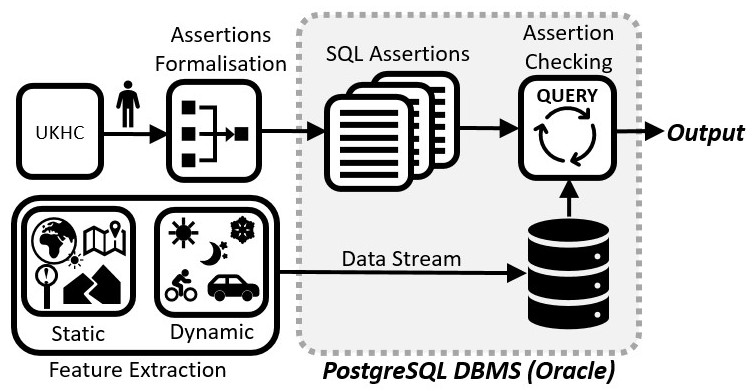
\includegraphics[width=0.98\linewidth]{\pathToOtherFiles/figures/SimulatorAssertionsCondensed.jpg}
    \caption{Testbench for interpreting and monitoring assertions.}
    \label{fig:SimulatorArchitecture}
\end{figure}



% GC added this as condensetion of section III **************
Figure~\ref{fig:SimulatorArchitecture} shows the testbench architecture that was used to formalise and monitor assertions and interpret the diving situation. The testbench is used by starting with the reference used to assess the driving situation, in this case the UKHC. Following this, there is a human-interpreted stage (human icon) that converts human-readable rules into formal assertions (\emph{Assertion Formalisation}) that are machine-readable. This forms one of two inputs to the \emph{Oracle} which uses postgreSQL database technology to perform the automated assertion checking. The second input to the Oracle is the \emph{Data Stream} of extracted features that is observing the driving scenario, which may be from simulation or from live sensor data. The \emph{Feature Extraction} process will capture relevant information from the driving scenario, including \emph{Static} elements such as the road network and \emph{Dynamic} elements such as vehicle position and orientation. Records are captured from the \emph{Data Stream} and stored on the PostgreSQL DBMS server at each available time step.
%
Automated assertion checking happens within the DBMS, where \emph{SQL Assertions} are stored which have been written to logically express the formalisations of the UKHC in the SQL language. At each time step the \emph{Assertion Checking} process executes a query engine that evaluates the relevant assertions encoded with the assertion logic against the stored records and generates a pass or a fail verdict as an \emph{Output}.



% GC removed this ************
% Figure~\ref{fig:SimulatorArchitecture} shows a layout for a simulation testbench that indicates the context in which the assertions database is used:
%   \begin{itemize}
%       \item During \emph{Experiment Instantiation}, specific test scenarios are generated from the \emph{Experiment Specification} which may include test objectives or requirements (defined in natural language). The Experiment Instantiation identifies the \emph{Static} information about the environment (e.g.\ maps, road features) and \emph{Dynamic} descriptions of the behaviour required of simulated actors (vehicles, other road users, traffic lights, and any third-party agents necessary to the test requirement). 
% %      The experimental configuration determines the test case that will contribute coverage towards the assertion.

%       \item The \emph{Simulator} interacts with the \emph{AV Control} - although for the purposes of this paper a dummy controller is used that can be set to pass or fail assertions to demonstrate the full extent of the assertion-based validation approach. The simulator used is the CARLA simulator\footnote{\url{https://carla.org/}}, but in principle this could be exchanged for other simulators with only moderate effort.
%       \item The \emph{Data Capture} records relevant simulation data about the driving situation of the AV, including actor positions and road network information, and at each time step of the simulation writes this information into the records of the database to be used for assertion checking.
%       \item The \emph{Assertion Checker} together with the \emph{Assertions} library constitute the test \emph{Oracle}. They evaluate all assertions relevant to the driving situation defined at each step of the simulation. 
%       \item The \emph{Outputs} are a set of Pass/Fail declarations.
% % which can be used to annotate the simulation log or be recorded in a separate file if desired. 
% \emph{Assertion coverage} with respect to the experiment specifications can also be monitored at the output. 
%   \end{itemize}
%   We will focus on describing the assertion oracle in greater detail in %the remainder of this paper
%   Section~\ref{geospatial_database}.

% \subsection{Operational Monitoring}
% The key observation motivating our approach to assertion-based monitoring during operation is that the assertions we have developed for assertion-based monitoring in simulation can also be utilised as runtime monitors during operation of a vehicle.
% %
% Thus, the same Assertions and Assertion Checker as those shown in Figure~\ref{fig:SimulatorArchitecture} can also be used in operational monitoring mode. The system architecture required to achieve this is illustrated in Figure~\ref{fig:RuntimeArchitecture}, wherein:
% \begin{itemize}
%     \item The \emph{AV Sensors} acquire real-time information from the vehicle's sensors.
%     \item During \emph{Feature Extraction}, the data obtained from the vehicle's sensors are processed to provide a trace that is equivalent to that obtained from simulations, so that the \emph{Assertion Checker} can be applied in operational mode.
%     \item \emph{Data Capture}: as in % the simulation environment in
%  Figure~\ref{fig:SimulatorArchitecture}, the data describing the vehicle's environment and observable actions is captured and stored in a database for  assertion checking.
%     \item The \emph{Assertion Checker} and \emph{Assertions} library are essentially identical to that of the simulation environment in Figure~\ref{fig:SimulatorArchitecture}, evaluating the relevant assertions and generating a pass or a fail verdict~\cite{RuntimeReview} as an output. 
% % KIE: taken out to shorten the paper, this can be said in the conclusion or under future work, perhaps. 
% % In some applications, there may be differences in the deployment (as shown in Figure~\ref{fig:RuntimeArchitecture}) compared to the simulation testbench, where the system would be deployed on embedded hardware. These applications include operational data recording for further processing or possibly its use as a real-time reward for online learning.
 
% \end{itemize}

% %However, to generate a verdict some sort of reference model is needed, which in this case are the PostgreSQL queries, to provide logical expressions of safety properties for what is to be classified as expected or unexpected behaviours (pass or fail) of the AV; and accordingly execute the appropriate steps to ensure safety.
 
% \begin{figure}[h!]
%     \centering
%     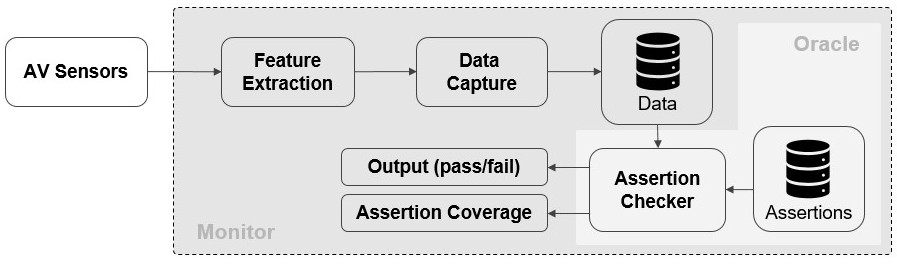
\includegraphics[width=0.98\linewidth]{\pathToOtherFiles/figures/RuntimeAssertionsTestBenchArchitecture.jpg}
%     \caption{Operational monitoring architecture}\todo[inline]{Revise to match new version of Fig. 1 almost exactly, i.e. replace AV Control with AV Sensors, replace Simulator with Feature Extraction, remove all above Simulator, leave rest as is. Done. :)}
%     \label{fig:RuntimeArchitecture}
% \end{figure}









\subsection{Geospatial Database for Assertion Checking} \label{geospatial_database}
To develop assertions derived from UKHC rules, we need a formal language into which they can be translated for automatic checking. Two aspects are important to the choice. First, as we discuss later, the rules and guidelines in the UKHC are written for human readers not automatic systems. They consist of sets of discrete rules applicable to specific aspects of road user behaviour, which must be taken collectively, and not necessarily always in a particular order, to form the legally required profile of behaviour. This suggests that a declarative programming language, such as Prolog or SQL, may offer the required expressive power for encoding rules.
%
Second, to process the data produced during driving, we seek languages that handle large data sets naturally, where the assertions constitute formal operations on datasets corresponding to the logical properties we extract from the UKHC rules. 
%
Taking these two requirements into consideration, SQL emerges as the most suitable programming language. SQL has been demonstrated formally~\cite{sqllibkin} to be sufficiently expressive to be able to encode related problems such as state or graph reachability as well as all standard problems in relational algebra, albeit with the use of some of its later extensions such as recursive operators. Safety properties can be defined in terms of reachability~\cite{guiochet2015, masson2019} or (in-)stability~\cite{harper2005, xue2020} of desirable (goal) and undesirable (hazardous) situated states. For these reasons, we have selected SQL-based database technology as the framework for our assertion-based oracle. 

The technical challenge then becomes how to compare the data captured against the assertions. We argue that a geospatial relational database is well suited for this purpose. The vehicle state can be easily stored and accessed. Additional insights, such as dynamic properties, can also be derived from this base information. 
% KIE taken out as this is expressed also in the next para:
% A database system, such as PostgreSQL, can record, access and perform assertion checks upon this state information quickly and reliably and is especially useful considering libraries that make use of geographical shape objects, e.g.\ PostGIS. 
%
Thus, we have implemented Assertion Checking as a PostgreSQL database with a PostGIS geospatial information system extension, which provides an extensive library of SQL-native spatial measurement functions. We chose these particular software products because they are open-source, and PostgreSQL implements powerful, high-performance table searching algorithms.
% - in the order of hundreds of thousands to millions of records searched per second. 
Real applications will involve the use of large data sets, so the performance of the underlying database engine is an essential factor in practice. % in achieving a practicable system.

% \begin{figure*}[h!]
%     \centering
%     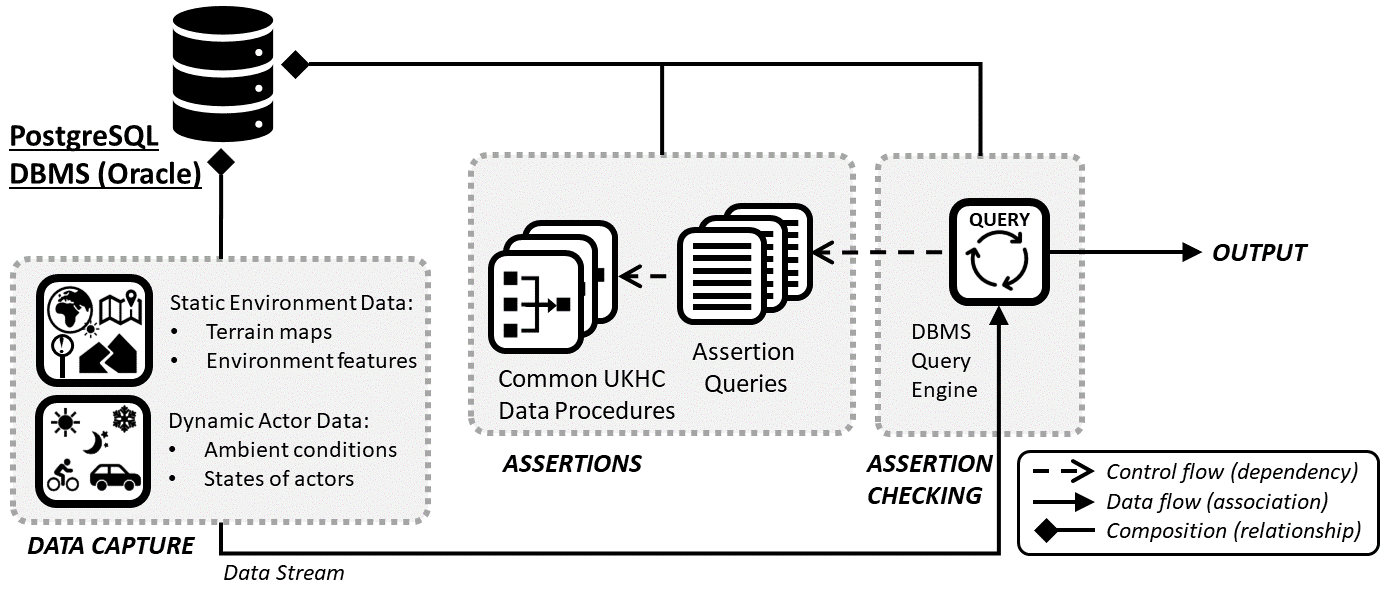
\includegraphics[width=18cm]{\pathToOtherFiles/figures/DBMS_deployment.png}
%     \caption{Deployment of the PostgreSQL DBMS, showing interactions with the Data Capture and Assertion Checking.}\todo{The DBMS is not the oracle. The Assertions and AC are the oracle together, see prev. figures. Please correct.}
%     \label{fig:dbms_deployment}
% \end{figure*}

% GC TODO replace references to fig:dbms_deployment

% KIE taken out to shorten paper
% The database management system (DBMS) receives data from the simulator (or other data source) containing an actor state vector of variables such as position, velocity and yaw angle of the vehicles and other road users (e.g. pedestrians). This data is then entered into a set of tables, and the safety assertions are applied to the data as one or more database queries (written in SQL) acting on the relation.

% Figure~\ref{fig:dbms_deployment} is a UML-style deployment diagram of the Data Capture and Assertion Checking functions using a PostgreSQL DBMS server. In fact, the server hosts both elements; the Data Capture function is implemented as a set of records that can be updated externally, e.g.\ by the Simulator or Experiment Instantiation functions; the Assertions Checking function is performed by the DBMS query engine by execution of SQL queries encoded with the assertion logic. 
%, potentially as a stored procedure, that will typically run all relevant assertions sequentially at each time step. 
% The assertions are stored in the database server as a set of SQL queries or procedural functions to be invoked by the query engine. 
% whenever required.

The use of PostGIS introduces an extensive library of data types and method functions suited to measurement of basic physical (geometric) relationships. For the overtaking scenario in this paper, functions measuring distance between geometric objects (the bounding-box shapes of vehicles on the road), and partial or total containment of the vehicle within road lane geometries, are of particular use to assess vehicle positions during the overtaking manoeuvre.

PostGIS functionality can also be used to generate more complex geometric dynamic data derived from the basic state of the vehicle or other agents. An example of this is shown in Figure~\ref{fig:assertion_database_annotated}, in which two polygons for \textit{thinking distance} (inset, green hashed area) and \textit{braking distance} (red hashed area), which are parameters defined in the UKHC (Rule 126), can be generated as a function of the basic forward velocity data of the vehicle. Figure~\ref{fig:assertion_database_annotated} shows a projection of these derived geometries onto the associated street map. 
%
Thus, new abstractions can be developed by deriving new data sets from the original (captured) data. These can be manipulated effectively as a new variable (SQL attribute) appended to the original data set, and referenced by queries in the same way.
%

% GC removed an included description above


This is an essential principle of our methodology. Procedures and queries can be developed to generate abstractions directly related to the concepts expressed in the rules of the UKHC. 
% The methodology for identifying assertions and key abstractions is described in Section~\ref{Use_of_assertions}. 
Where such concepts are used in multiple rules, the corresponding abstractions form a library of common queries or operations on data, which can be incorporated into the PostgreSQL DBMS. % as a set of stored procedures within the general database schema.
%
% GC shortened this section
% Figure~\ref{fig:dbms_deployment} shows how the procedure library is included in the overall deployment and its dependencies to other elements of the system. This library will be developed incrementally as each assertion is produced. We anticipate that eventually the library of procedures may be packaged and made available as a PostgreSQL extension. \todo{KIE: .tex para could be removed to shorten paper.} Data and derived abstractions can be combined within queries for assertion checking and coverage collection. For example, an assertion to determine whether the braking zone of the AV has intersected another road user, such as a vehicle travelling in the opposite direction, can be formulated as PostgreSQL query:
%
%\begin{lstlisting}[
%           language=SQL,
%           showspaces=false,
%           basicstyle=\ttfamily,
%           numbers=none,
%           numberstyle=\tiny,
%           commentstyle=\color{gray}
%           ]
%        
%SELECT ST_Overlap(g1.geom::geography,
%                   g2.geom::geography)
%FROM sim_log.data g1
%WHERE g1.agent_id = AV_braking_zone 
%AND g2.agent_id = Oncoming_Vehicle;
%\end{lstlisting} 
%
%where a PostGIS library function, \texttt{ST\_Distance}, is used to measure the shortest Euclidean distance between the two physical objects or geographical areas g1 and g2, which are a vehicle braking zone and an oncoming vehicle.\todo{KIE: This does not use ST\_Distance? Note, this example could potentially be removed to shorten the paper. }

\begin{figure}
    \centering
    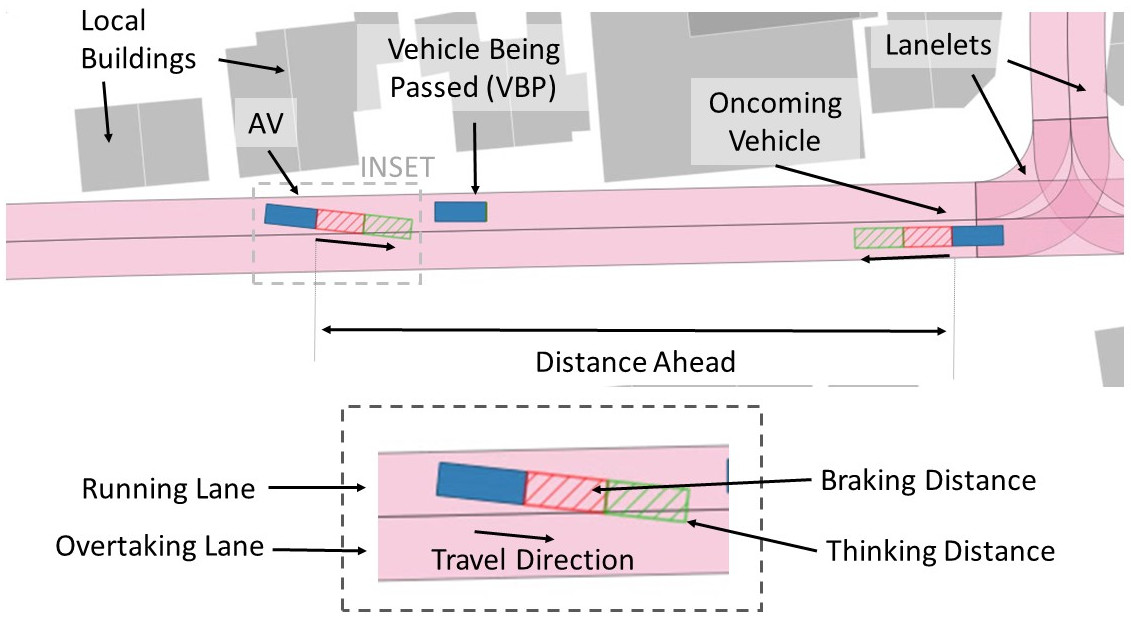
\includegraphics[width=8.5cm]{\pathToOtherFiles/figures/assertion_database_annotated.jpg}
    \caption{Database view of a driving scenario.}
    \label{fig:assertion_database_annotated}
\end{figure}

To illustrate the functionality of the PostgreSQL DBMS server, Figure~\ref{fig:assertion_database_annotated} shows the operating situation associated with the overtaking scenario described in Section~\ref{Experimental_scenario}, and gives an example of a derived variable called \emph{Safe Distance Ahead} (SDA), whose name is derived from terminology in Rule 162 of the UKHC. The figure shows an urban scene depicting a section of road network divided into \emph{lanelets} denoting legal division between driving lanes and any buildings in the area. In this example the AV is on the left of the figure overtaking a parked vehicle requiring a lane change. The distance to the oncoming vehicle is termed the Distance Ahead. The inset shows annotation denoting the braking and thinking distances of the AV which can be treated as geographical object entities in the database and hence easily used for assertion checking. 

The assertion performs a check (as defined in UKHC Rule 162) that a safe distance ahead exists between an AV and the nearest vehicle in an oncoming lane, labelled the `Oncoming Vehicle' (OV) as the AV starts to overtake the `Vehicle Being Passed' (VBP). The start time of the overtake is defined as the time that the AV first begins to enter the adjacent lane (Overtaking Lane) of the road, at which point it must commit to the manoeuvre or else abort and return to driving in the initial lane (the Running Lane).

In the case of assertions related to overtaking, it is necessary to determine whether the overtaking vehicle wholly or partly occupies a given road lane, since overtaking manoeuvres require it to move at least partially into an adjacent lane and back. Therefore, it is necessary for the database to include lane geometries (polygons) in order to allow checking of vehicle occupancy of lanes by testing for the overlap between vehicle and lane objects. Figure~\ref{fig:assertion_database_annotated} shows the lane polygons projected onto the map section (an extract from the map used for our initial assertion checking experiments described in Section~\ref{Experimental_scenario}). The start of an overtaking manoeuvre is identified as the first time step in which the vehicle overlaps the overtaking lane (and stops being wholly contained within the running lane), and the overtake manoeuvre ends when the vehicle is entirely within the running lane once more after having passed the VBP. Lane geometry objects (shape or bounding box polygons) are therefore an essential element of the assertions related to overtaking.











\section{Assertion Development and Application}\label{Use_of_assertions}
In this section we first identify the types of assertions that may exist. We then discuss how to develop assertions from the natural language statements of the UKHC. We also present how to use assertions, both in simulation and during operation.

\begin{figure}[!b]
    \centering
    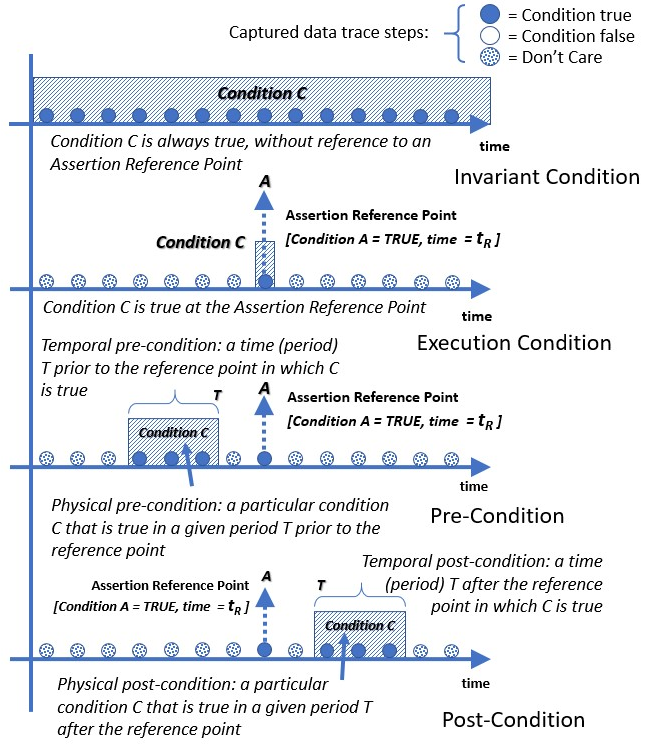
\includegraphics[width=0.98\linewidth]{\pathToOtherFiles/figures/Assertion_Categories_Figure.png}
    \caption{Types of assertions.}
    \label{fig:categories_of_assertions}
\end{figure}


\subsection{Types of Assertions} \label{assertion_categories}

The assertions to encode UKHC rules tend to fall into one of four principal types. Except for invariants, assertions are defined with respect to some \emph{assertion reference point} - a particular step of a captured data trace, defined by some reference condition which holds at a specified time step. The assertion is then defined as some spatio-temporal condition relative to the reference point, as shown in Figure~\ref{fig:categories_of_assertions}.


The four types of assertions are:
\begin{itemize}
    \item Invariant Condition: A condition that must be satisfied at all time steps within the captured data trace.
    % (i.e.\ there is no specific assertion reference point, or the reference point is in effect the entire trace).
    \item Execution Condition: A condition that must be satisfied at the assertion reference point.
    \item Pre-condition: A spatio-temporal phenomenon that must exist in the steps preceding the assertion reference point. 
    \item Post-condition: A spatio-temporal phenomenon that must exist in the steps following the assertion reference point.
\end{itemize}

Pre-conditions and post-conditions can be one of two sub-types:
\begin{itemize}
	\item \textit{Temporal}: A time period preceding or following the assertion reference point, within which a specified condition holds. This is the temporal component of the overall spatio-temporal condition. Examples include:
	\begin{itemize}
		\item \textit{Temporal pre-condition: as a vehicle crosses a highway exit lane boundary (reference point) an assertion checking that the vehicle's indicators have been set continuously in a preceding period (e.g.\ 5s) (i.e.\ checking for unduly late or intermittent indications).}
		\item\textit{Temporal post-condition: a highway exit assertion may check that if a vehicle starts indicating to leave at the exit lane, then it does enter the exit lane within a given time period (i.e.\ checking for unnecessarily early indications).}
	\end{itemize}
	
	\item \textit{Physical}: A physical (e.g.\ spatial or state) condition that must be satisfied at a specified time(s) before or after the assertion reference point. This is the physical component of the overall spatio-temporal condition. Examples include:
	\begin{itemize}
		\item \textit{Physical pre-condition}: a check that, as it passes the exit lane boundary, a vehicle's indicators were set at the last highway exit sign before the exit (i.e.\ checking for omitted indications).
		\item \textit{Physical post-condition}: a check that if a vehicle is indicating to leave in the approach to an exit lane, then it does in fact leave the lane (i.e.\ this is a check for false or spurious indications).
	\end{itemize} 
\end{itemize}

% this following paragraph has not yet been revised, but should be updated to reflect the changes in the previous few paragraphs - TBD by Chris
\subsection{The importance of selecting relevant assertions} \label{assertion_triggers}
Identifying which assertions are relevant in a given situation is important to manage the performance of assertion checking and to ensure the output is meaningful. For example, assertions checking highway driving behaviour are not applicable in urban or rural road environments, and may cause confusion if applied in inappropriate contexts. 
Similarly, different assertions checking for mutually exclusive conditions will be guaranteed to generate errors unless the inappropriate assertions are filtered out. For example, checking that an AV is braking smoothly will inherently fail in a situation where it is required to accelerate. If assertions of this kind are not selected correctly, they will generate nuisance failure results. 

Filtering assertions can also improve real-time performance of the simulator when they are being applied in a more time-critical mode of operation - for example  simulation control (see Section \ref{Assertions_at_Sim_Time}). If the assertion type can be embedded in its script (for example, in its header), then the Assertion Checking process in the Testbench (see Figure~\ref{fig:SimulatorArchitecture}) can be set to check only assertions of a given type.

Discrimination or pre-selection of assertions can also be achieved by specifying `trigger conditions' based on the type of \textit{Operating Design Domain (ODD)} in which the assertion is relevant.
\footnote{This is similar to typical practice in computer hardware verification \cite{tao2009}, where an assertion may take the form ``under $<$environment conditions$>$ if $<$trigger$>$ then $<$expectation$>$", where \textit{$<$environment conditions$>$} may be ``we are not in RESET mode" and \textit{$<$trigger$>$} may be ``we receive a request" and \textit{$<$expectation$>$}  may be ``an acknowledge signal is driven high sometime in the X next cycles".} 

%Category codes for these types have been embedded in the header information of each assertion source code file. This allows the %simulator
%test-bench system to select automatically which types of assertions to run, depending on the mode of operation of the Assertion Checking subsystem %during a simulation run 
%(see Section \ref{Assertions_at_Sim_Time} ). If runtime %dynamic
%assertion checking is required, then the %simulator
%system can opt to apply only the invariant and execution conditions, %leaving the pre- and post-condition assertions (which may have greater %processing overheads) to be applied retrospectively after the data log %has been fully captured. %simulation run has been completed.

\subsection{Deriving machine-oriented logical assertions from human-oriented Highway Code rules}
Developing assertions from the UKHC - a natural language developed for human readers - requires that it be interpreted in a consistent manner; we present two approaches to constructing logical assertions from the text. 

\subsubsection{Interpretation of Natural Language UKHC Rules} \label{interp_nat_lang_UKHC_rules}

The UKHC comprises several hundred rules and guidelines, applicable to different categories of road user (including those on foot - pedestrians, cyclists, horse riders - as well as the usual cars, vans, or trucks and buses) and covering a number of different aspects of road use (including general driving advice, instructions for maintenance and repair of vehicles, and instructions for management of situations such as emergencies). The UKHC rules are written entirely for human readers, and seek to offer guidance in common sense terms that any reader should understand clearly. For example, two rules of central interest to this paper relate to overtaking manoeuvres:

\begin{quote}
    \underline{Rule 162}
    
    \textbf{Before overtaking} you should make sure
    \begin{itemize}
        \item the road is sufficiently clear ahead
        \item road users are not beginning to overtake you
        \item there is a suitable gap in front of the road user you plan to overtake.
    \end{itemize}
	\vspace{8mm}	% This vspace pushes the Rule 163 title onto the next page alongside the rule text - looks neater. Modify or delete as needed if the text gets reformatted.
    \underline{Rule 163}
    
    \textbf{Overtake only} when it is safe and legal to do so. You should
    \begin{itemize}
        \item not get too close to the vehicle you intend to overtake
        \item use your mirrors, signal when it is safe to do so, take a quick sideways glance if necessary into the blind spot area and then start to move out
        \item not assume that you can simply follow a vehicle ahead which is overtaking; there may only be enough room for one vehicle
        \item \emph{move quickly past the vehicle} you are overtaking, once you have started to overtake. \emph{Allow plenty of room. Move back to the left as soon as you can but do not cut in}
        \item take extra care at night and in poor visibility when it is harder to judge speed and distance
        \item give way to oncoming vehicles before passing parked vehicles or other obstructions on your side of the road
        \item only overtake on the left if the vehicle in front is signalling to turn right, and there is room to do so
        \item stay in your lane if traffic is moving slowly in queues. If the queue on your right is moving more slowly than you are, you may pass on the left
        \item give motorcyclists, cyclists and horse riders at least as much room as you would when overtaking a car (see Rules 211 to 215).
    \end{itemize}
\end{quote}

This example illustrates several characteristics found frequently in UKHC rules:
\begin{enumerate}
    \item Rules are often expressed in a second-person tense, offering advice directly to the reader. Converting them into assertions that are in effect performed (measured) from an external third-person perspective requires changes that may transform the logic of the rule to some extent.
    
    \item The logical sense of the safety property expression (i.e. whether the rule expresses a pass or a fail condition) varies depending on the concept being expressed. Since the general guidance for direct conversion of rules is to keep as close as possible to the top level natural language, the logical sense of the assertions will follow suit. This contrasts with typical practice for their use in conventional computer programming, where the standard practice is to encode an assertion such that a pass condition permits a program to continue running normally, and a fail causes an exception to be triggered.
    
    \item Being written at a natural human-readable level of abstraction, the rules and guidelines rely greatly on the reader having sufficient background knowledge and capability to resolve their generalized constraints to the point where actions can be selected that satisfy them.
    
    This abstraction also interferes with the ability to validate the assertions by any means other than manual design review; formalization of the assertions may require all the hidden complexity to be reintroduced.
    
    \item Many clauses of UKHC rules offer advice to drivers about their internal decision making, often in the form of constraints. The third bullet-item of Rule 163 is a typical example. These clauses cannot be measured externally without some form of communication by the driving agent (for example, an AV) of the results of its decision-making processes. To date we have not attempted to establish assertions of this kind, as there are no standards or conventions by which an AV might explain and communicate its actions. However, we note that this is an interesting direction of future work (see Section \ref{discussion}). 
\end{enumerate}

Two methods have emerged for developing assertions from the UKHC: direct translation into logic, and the use of modelling. These are discussed in the next subsections.

\subsubsection{Method 1: Direct translation into logic} \label{direct_translation}

The basic approach involves simply converting the natural language text into a logical predicate. We developed a procedure containing the following steps: 
\begin{enumerate}
    \item \emph{Identify and extract a given UKHC rule clause.} 
    \begin{itemize}
    	\item A separate assertion will be required for every distinct subject-verb-object clause in the text; a given UKHC rule could easily require on the order of 5-10 separate assertions to be fully covered;
    	\item the clause must define a \emph{testable} requirement - some UKHC rules are (at least at present) not testable. [We discuss this issue further in Section \ref{discussion}.]
    \end{itemize} 
    \item \emph{Write a natural language hypothesis that captures the safety property of the rule.} 
    \begin{itemize}
    	\item A useful way to do this is to phrase the natural language hypothesis interrogatively, i.e. as a question.
    	\item Many rules are written imperatively, as orders or advice for road users to follow. The associated hypothesis is straightforward: were the conditions of the instruction(s) satisfied?
    \end{itemize}
      
    \item \emph{Write a logical statement that reflects accurately the assertion hypothesis}
    \begin{itemize}
    	\item Note that the perspective of the hypothesis may need to be transformed to a 'third-person' (external) point of view.
    	\item Write the assertion logic as closely as possible to the language of the assertion hypothesis, keeping the same high-level terms (These can then be elaborated and evaluated as stored procedures in the database management system, as discussed in Section \ref{generic_sim_system}) 
    \end{itemize}
   
    \item \emph{Verify assertion logic correctness by manual design review.} 
    \begin{itemize}
    	\item As previously mentioned, pragmatically this is the only method available. But if the assertion logic is directly comparable to the  natural language of the assertion hypothesis, this step should be reasonably self-evident.
    \end{itemize}
    
\end{enumerate}

As an example of the direct translation method, consider the following clause from UKHC Rule 258. The procedure could be applied as follows:

\begin{itemize}
    \item \emph{UKHC rule clause:}
	    \begin{quote}
			\textit{\textbf{Red flashing lights.} If red lights flash on a signal and a red `X' is showing, you MUST NOT drive in the lane shown as closed beyond the signal.}
		\end{quote}
    \item \emph{Assertion Hypothesis:}
        \begin{quote}
        	The hypothesis question is: \textit{Does the AV pass a `Lane Closed’ overhead gantry signal?}
        \end{quote}
    \item \emph{Assertion Statement (Predicate logic):}
         The assertion question concept of passing a sign then becomes a test of whether the AV bounding-box geometry overlaps with a boundary line between the posts of an overhead gantry object, which must lie across the roadway.
               
         This can be converted into an SQL query (SELECT statement) returning all time steps where the bounding box shape of a vehicle overlaps the line between the posts of an overhead gantry and the overhead sign of that gantry reads "Lane Closed" for the road lane occupied by the vehicle.      
         \footnote{Note: this skeleton SQL schema is an illustrative example only and was not tested experimentally. The experimental results presented in section \ref{Experimental_scenario} are based on a clause from UKHC Rule 162 on overtaking.}\\
\scriptsize    %scriptsize gets all the SQL code into a column width
\begin{lstlisting}[
           language=SQL,
           showspaces=false,
           basicstyle=\ttfamily,
           numbers=none,
           numberstyle=\tiny,
           commentstyle=\color{gray}
        ]
SELECT (time, ST_Overlap(AV.geom::geography,
    	      GantryLine::geography) ) ASC LIMIT 1
FROM simulation_data AS sd
WHERE
  sd.agent_id = /* the AV's ID */ AND
  RoadType(sd.agent_id) = 'ATM_MOTORWAY' AND
  LaneStatus(sd.agent_id) = 'LANE_CLOSED' AND
  GantryLine = FindNextGantryLine(agent_id);
\end{lstlisting}
\normalsize %normalsize resets the font size
Key concepts of the assertion (for example, boundary lines of overhead gantry signals) become predicates in the assertion logic, and can be implemented as SQL procedural functions stored in the PostgreSQL database (refer back to Section \ref{generic_sim_system}).

We anticipate that typically assertion queries will make use of PostGIS relational operators and functions for object geometries, whereas the library functions will typically use PostGIS geometry constructors to set up the geometric objects for the assertions as variables derived from the captured simulation data (as discussed in Section \ref{generic_sim_system}). A hierarchical organization of queries and procedural functions (from Assertions to CAV DBMS library functions to PostGIS functions to captured simulation data) emerges from this approach.\\
\end{itemize}

\subsubsection{Method 2: Model-based Analysis} \label{model_based_analysis}

While many UKHC rules can be translated directly into logical conditions or constraints expressible as simple Boolean predicates, some describe more complex situations that may require more explicit modelling to identify the assertion hypothesis and logical expression. We require no particular constraints on the modelling methodology used, except that it needs to produce a well formed logical expression deriving the essential parameter of the assertion hypothesis from the captured data trace of the simulation.

As a worked example, we present an assertion we developed from Rule 162, which we applied experimentally as discussed later in Section \ref{Experimental_scenario}.
The first two steps of this method are the same as for Method 1: identify the UKHC clause and the associated assertion hypothesis:
\begin{itemize}
	\item \emph{UKHC rule clause:}
		\begin{quote}
			\textit{Before overtaking you should make sure the road is sufficiently clear ahead.}
		\end{quote}
	\item \emph{Assertion Hypothesis:}
	\begin{quote}
		The hypothesis question is:
		
		 \textit{Is the distance between the AV and OV sufficiently large to complete the overtake manoeuvre, at the moment the AV starts it (i.e.\ as it crosses the road centre line into the overtaking lane)?}
	\end{quote}
\end{itemize}
While the UKHC rule clause seems straightforward, the natural language actually encapsulates a complex judgement that a vehicle driver must make at the moment they begin an overtake manoeuvre. The driver must judge whether the distance between their vehicle and any oncoming vehicle in the adjacent road lane is sufficient to allow the manoeuvre to be completed safely. This is contingent on the (relative) speeds of the driver's vehicle (the AV), VBP and OV, line-of-sight distances to limits of view or obscuring obstacles such as bends in the road, blind summits, or road-side buildings, as well as the style of manoeuvre that the driver intends to perform - an `aggressive' overtake manoeuvre can probably be completed in less distance than a `relaxed' one~\cite{decastro2018counterexample, tkachenko2018line}.\footnote{The internal plans and intentions of an AV may not be available to the external validation system, so the definition of the assertions may need to make default assumptions about its intentions, or make a `worst case' test that checks against the most conservative case that can be assumed. For example, using the case of Overtaking, the assertion could assume that the AV was making a `relaxed' overtake manoeuvre, in which case an assertion might register a safety violation for anything less than large separation distances between the AV and oncoming vehicle at the start of the manoeuvre, even though the manoeuvre could probably be completed safely if a more urgent profile were performed.} There is a complex relationship between all the elements of this assertion that is quantitative in nature and hence an algebraic formula must be developed that expresses the assertion hypothesis. Such expressions must be developed by modelling the situation.

%deriving formulae for distances covered by the AV as a function of the relative position and velocity of the other actors in the scenario (VBP and OV) in each segment of the manoeuvre. The model divides the whole overtaking manoeuvre into three distinct phases

In the case of this Rule 162 example, it was necessary to develop a complete model of the overtaking manoeuvre in order to produce an expression for the \emph{Safe Distance Ahead} (SDA), which calculates how far away the Oncoming Vehicle needs to be from the AV for an overtaking manoeuvre to be conducted without risk of collision. The analysis decomposed the overtaking manoeuvre into several stages: Pulling Out (into the oncoming lane), Passing the VBP, and Cutting In (to the original running lane). A formula was developed for the overall distance required to complete the manoeuvre without violating safety constraints (such as impingement upon vehicle thinking or braking distance (see Figure~\ref{fig:assertion_database_annotated}) or clearance distances around the VBP). 

A diagram of the full analysis model, and the derivation of the formula for Safe Distance Ahead, is provided in Appendix A. 

%For the purposes of describing the general approach we describe the analysis of one of the way points as a typical example. 

%The second waypoint is set at the transition from pull-out to passing the VBP, as shown in Figure~\ref{fig:Passing_t1}. The figure shows the expressions for the distance travelled by all vehicles in the \textit{$[t_0, t_1]$} time period (taking into account aspects such as the movement of the AV into the oncoming traffic lane):
% \begin{figure}
%    \centering
%    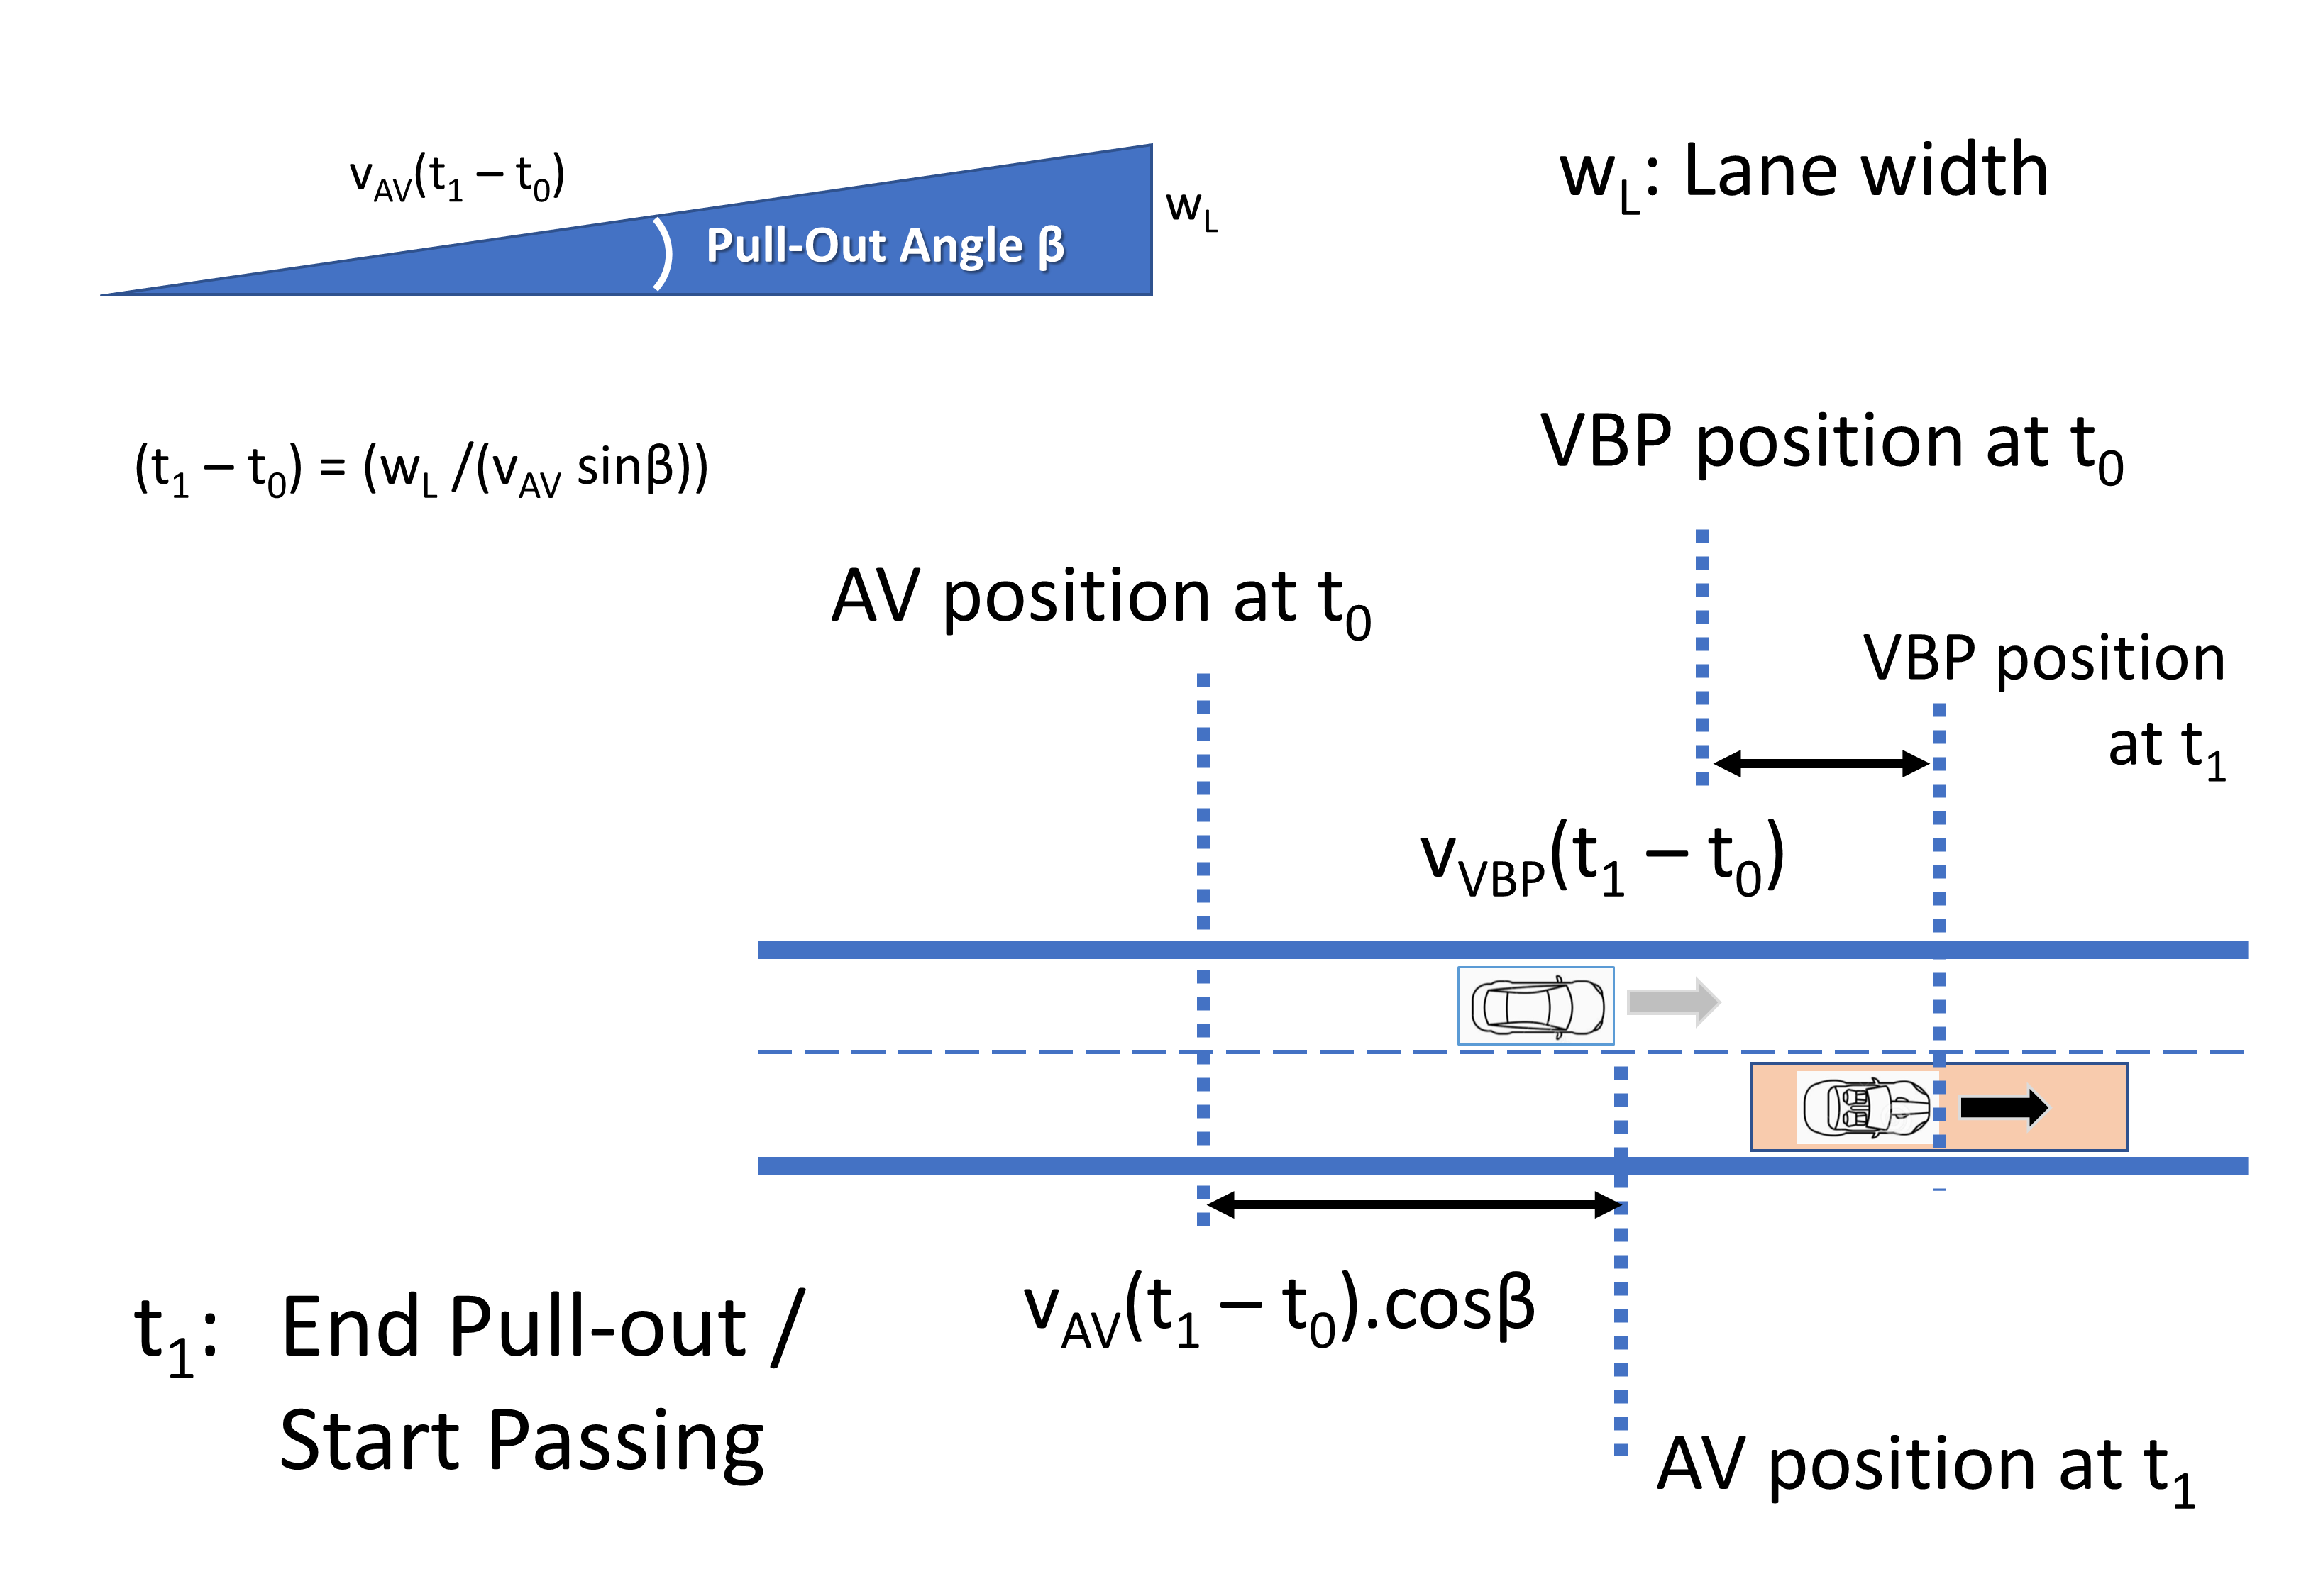
\includegraphics[width=0.98\linewidth]{\pathToOtherFiles/figures/Passing_t1_v2.png}
%    \caption{Scene as the AV begins to pass the VBP, time = $t_1$.}
%    \label{fig:Passing_t1}
% \end{figure}

%The overtaking manoeuvre analysis in Appendix A derives expressions for distance covered by each vehicle in the time periods between each waypoint, and hence a formula for the Safe Distance Ahead at time $t_0$ can be constructed by summing all the distances covered by the AV and the OV

The analysis identifies several key characteristic parameters that characterise the overtaking manoeuvre. These include:
\begin{itemize}
    \item \emph{Stopping distance} (SD) is defined as the sum of the `thinking distance' and `braking distance' of the vehicle (assuming it has a human driver) as defined in UKHC Rule 126 and illustrated in Figure~\ref{fig:assertion_database_annotated}.
    % 
    A table of the typical stopping distances for travelling speeds ($v$) between 20 mph - 70 mph is provided with Rule 126 in the UKHC.
    %
    Equation~\ref{DS_equation_rule126} is a regression formula derived from this table to estimate the stopping distance ($m$) given the vehicle speed ($mph$).\footnote{Refer to \url{https://www.gov.uk/guidance/the-highway-code/general-rules-techniques-and-advice-for-all-drivers-and-riders-103-to-158}} The coefficients are: $a=0.300$, $b=0.058$, $c=-0.011$ and $d=0.015$.
    
\begin{equation} 
\label{DS_equation_rule126}
\text{SD} = \underbrace{av }_{\substack{\text{Thinking} \\ \text{Distance}}} + \underbrace{b + cv + dv^2}_{\substack{\text{Braking} \\ \text{Distance}}}
\end{equation}

    \item \emph{Danger Space} (DS) is an area projected forward in the direction of travel with a length equal to the stopping distance and a width equal to that of the vehicle. The overall formula for SDA incorporates the DS of the OV.
    %
    SD varies with vehicle speed, making the DS a function of speed, therefore intuitively as the speed increases the DS ahead of the vehicle will project further forward accordingly.
    
    \item \emph{Pull-out Clearance} distance is the minimum safe separation that must be maintained as the AV pulls out into the oncoming lane (and carries its own constraints (and assertions) as defined in the first bullet-point of Rule 163 - see Section \ref{interp_nat_lang_UKHC_rules}).
    
    \item \emph{Pull-out Angle} ($\beta$) is the steering angle taken by the AV as it moves into the oncoming lane.
    
    \item The \emph{Cut-in Clearance} distance is the minimum required separation distance between AV and VBP when the AV begins to cut back into the running lane.
    
    \item \emph{Cut-in Angle} ($\theta$) is the steering angle taken during the cut-in move.
\end{itemize}

Taken as an ensemble, the last four parameter values in the above list define a \emph{driving profile} for the manoeuvre, which characterise  (informally) a level of urgency or aggression associated with the manoeuvre. An `aggressive' profile might be taken as one which has a low pull-out clearance, high pull-out angle, low cut-in clearance and high cut-in angle, indicating a `sharp and close' manoeuvre taken by the AV around the VBP. A more `relaxed' driving profile may have larger clearances and lower steering angles. Various profiles of manoeuvre with different characteristic values are assessed in the experimental work discussed later. It should be noted that other UKHC rules place (at least qualitative) restrictions on these parameters to ensure safe driving behaviour (see the fourth bullet-point of Rule 163 in Section \ref{interp_nat_lang_UKHC_rules}, and also Section \ref{sim_case_study}). 

As with the problem of direct translation of the UKHC rules, the approach aimed to develop a model using the concepts of the natural language of the rule rather than by other parameters, for example time-to-collision, which has been found in human factors studies to be the most significant parameter characterising overtaking manoeuvres \cite{lenard2018, Chen2015}. Hence the model developed for the Safe Distance Ahead measurement differs to many that have been developed for analysis of overtaking manoeuvres, which aim to capture the decision making of the driver rather than the characteristics of the legal code of behaviour that is essentially an independent observer's perspective on the scenario.

\subsubsection{Geospatial Database for Assertion Checking}
Analysis of the overtaking manoeuvre problem fits neatly into the geospatial database framework for assertion checking. The vehicles can be represented as shape objects using the PostGIS system extension which allows for logical tests and measurement metrics to be efficiently calculated between shapes. An Entity Relation Diagram (ERD), Figure~\ref{fig:erd}, shows the variables within the database structure and the relationships between them \footnote{See \url{https://en.wikipedia.org/wiki/Entity-relationship\_model} for an explanation of \textit{crow's foot} notation.}. 

For each log file there exists an environment table containing map information, which in this case is based on the openDrive\footnote{\url{https://www.asam.net/standards/detail/opendrive/}} and lanelet formats. From the lanelet data we derive a table containing useful entries such as lane width and orientation for the environment. Data captured from the simulation (or real-time monitor), contains a state vector for the actors in $data\_capture.actor\_state$ which contains position and orientation information. From this captured data table we can calculate dynamic state information, that is information changing over time (e.g. velocity, acceleration) or with vehicle speed (e.g. braking distance). 

Further insight to the driving situation can be derived when combining actor state information with information about the environment. For example, driving lane orientation ($lanelets.lane\_orientation$) can be used to calculate the vehicle heading angle relative to the driving lane, to infer the cut-in or pull-out angles ($state\_dynamics.pull\_out\_angle$) required for the Safe Distance Ahead calculation. The final $assertions$ table is where the Safe Distance Ahead test output can be written and stored as a Boolean pass/fail result.

\begin{figure}
    \centering
    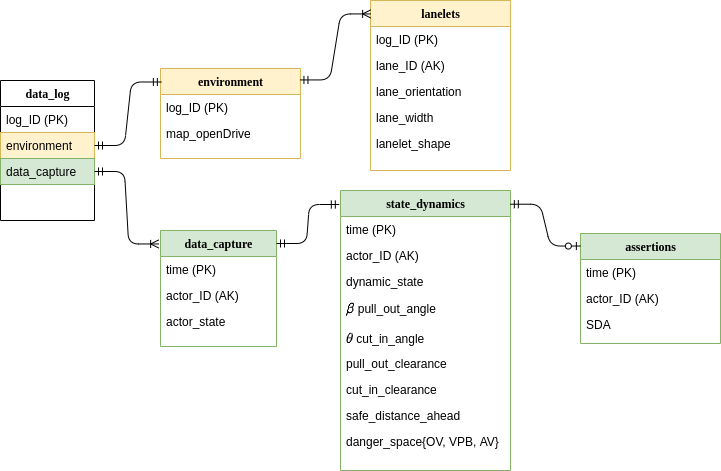
\includegraphics[width=8.5cm]{\pathToOtherFiles/figures/ERD2.png}
    \caption{PostgreSQL database Entity Relationship Diagram.}
    \label{fig:erd}
\end{figure}


\subsection{Modes of Use of the Assertion-checking Subsystem} \label{Assertions_at_Sim_Time} \label{assertions_at_run_time}

Assertion-checking databases can be used as a test oracle (see Sections \ref{generic_architecture}) in a variety of ways, both during simulation and in runtime monitoring:
\begin{itemize}
	
	\item \underline{\textbf{Modes of use during simulation:}}
	
	\begin{itemize}
		\item \emph{Simulation Control(Halting)}: Assertions can be checked as the simulation runs, and a simulation could be halted after a major safety violation if there is little value in continuing with a simulation beyond that point.
		
		\item \emph{Operator Warnings}: As above, assertions can be checked as the simulation runs, but instead of halting the operator can be warned of the occurrence, allowing them to exercise their judgement on whether to continue.
		
		We anticipate that this may be the best policy for minor safety violations or events such as collisions which may lead to secondary effects like non-deterministic behaviour in the simulator \cite{chance2021}, where the log file data might be degraded or unrepeatable following the event. The simulation may need to be halted, but pragmatically we believe this decision is probably best left for test engineers to decide. However, the use of assertions to provide operator warnings could be a beneficial mode of use.
		
		\item \emph{Simulation Log Annotation}: for negligible safety assertions failures, or for non-safety checks such as service performance monitoring, assertions could be checked as the simulation runs. But, instead of halting or providing warnings, assertion failures could simply result in annotations being added to the simulation log data, indicating that an assertion failed at a given time step but otherwise having no other externally observable effect. The log can then be analysed retrospectively after the simulation run has finished.
		
		\item \emph{Retrospective analysis}: Instead of checking assertions as the simulation runs, the captured data can be recorded and passed to the assertion checking database after simulation has finished, to analyse an AV's performance retrospectively. To date this is the mode in which we have been using the assertion-checking facility.
	\end{itemize}

	The simulation experiments with assertions presented in Section \ref{Experimental_scenario} were all run retrospectively, as they were a simple demonstration of concept rather than full implementation of the above modes of use. In the ongoing development of the simulation pipeline at Bristol Robotics Laboratory, we are focusing on the retrospective mode of use initially, as this represents the least complex software development option, and will then proceed to enabling dynamic checking during simulation time once this basic mode of operation has been demonstrated.\\ 

	\item \underline{\textbf{Modes of use during runtime monitoring:}}
	
	\begin{itemize}
		\item \emph{Warnings and Alarms}: Assertion checks can be used to raise warnings or alarms to human vehicle operators, to draw their attention or request them to take control over the vehicle if safety violations occur. 

		Additionally these warnings can be used to indirectly assess the performance of subsystems in an AV during operation to provide feedback for further development in future versions of the system.
		
		\item \emph{Triggering safety functions}: Detection of assertion violations can be used to initiate automated pre-planned risk mitigation plans as a safety function, where such occurrences present an immediate and sufficiently high risk that such a reaction is warranted ~\cite{RuntimeReview}. Having a ground truth reference to judge on monitored data at runtime can be challenging. Assertion failures can provide a reliable verdict to help AVs execute appropriate risk mitigation plans.
		
		\item \emph{Self-adaptation}: using assertion checking during runtime can be combined with measurements of key performance indicators (KPIs) and safety performance indicators (SPIs)~\cite{Koopman2020} or other scoring functions to help the AV (or autonomous systems more generally) to actively learn and reliably adapt their behaviour during operation (\cite{Kang2020}).
		
		\item \emph{Accident investigation or insurance risk assessment}: Assertion-checking subsystems can be used to annotate the internal data logs of an AV to help identify potential causes of an accident in any post-incident investigation (similar to flight data recorders in aircraft), or to measure the occurrence rate of UKHC driving rule infractions for insurance risk adjustment purposes. However, there are ethical concerns associated with such applications, as discussed in ~\cite{EthicalBlackBox}.
		
	\end{itemize}
\end{itemize}


\section{Experimental Case Studies} \label{Experimental_scenario}
As an aid to developing the methods and techniques described previously, we created some worked examples of assertions and measurements applied both to simulation data and real-time video footage. The experiments were early stages of work in developing the methodology, and were not developed by all the methods described in this paper, nor possess all the features described herein, but they did guide the development of the methodology and we believe that they do prove the general concept and utility of the approach. The use of methods such as modelling, and the need for features such as the use of standard procedures/library functions, all emerged as direct consequences of these experiments.

We chose two case studies inspired from a challenging overtaking scenario; the first aims at demonstrating the use of assertions in simulation testing, and the second shows how assertions can be used as SPIs or monitors to assess the safety performance of an AV or other road users during runtime.

\subsection{Experimental Scenario} % (from the NHTSA/CARLA Challenge)}
\label{carla_challenge}
To demonstrate the functionality of the assertion based safety validation process, we chose to consider an overtaking scenario similar to Scenario 6 of the driving situations in the NHTSA\footnote{\url{https://www.nhtsa.gov/}} pre-crash typology~\cite{nhtsa_precrash} that were published in the CARLA Challenge\footnote{\url{https://carlachallenge.org/}} The corresponding UKHC rules \cite{highwayCode} that apply to this scenario are Rules 162-169. Specifically, the scenario involves overtaking on a single-lane road where the test vehicle must perform a lane change to avoid a parked or broken down vehicle. 
% , Figure~\ref{fig:carla_challenge_NHTSA_task6_LHS}. 
The vehicle must leave sufficient gap to the vehicle it is overtaking and also not endanger any vehicles that are oncoming.

% \begin{figure}
%     \centering
%     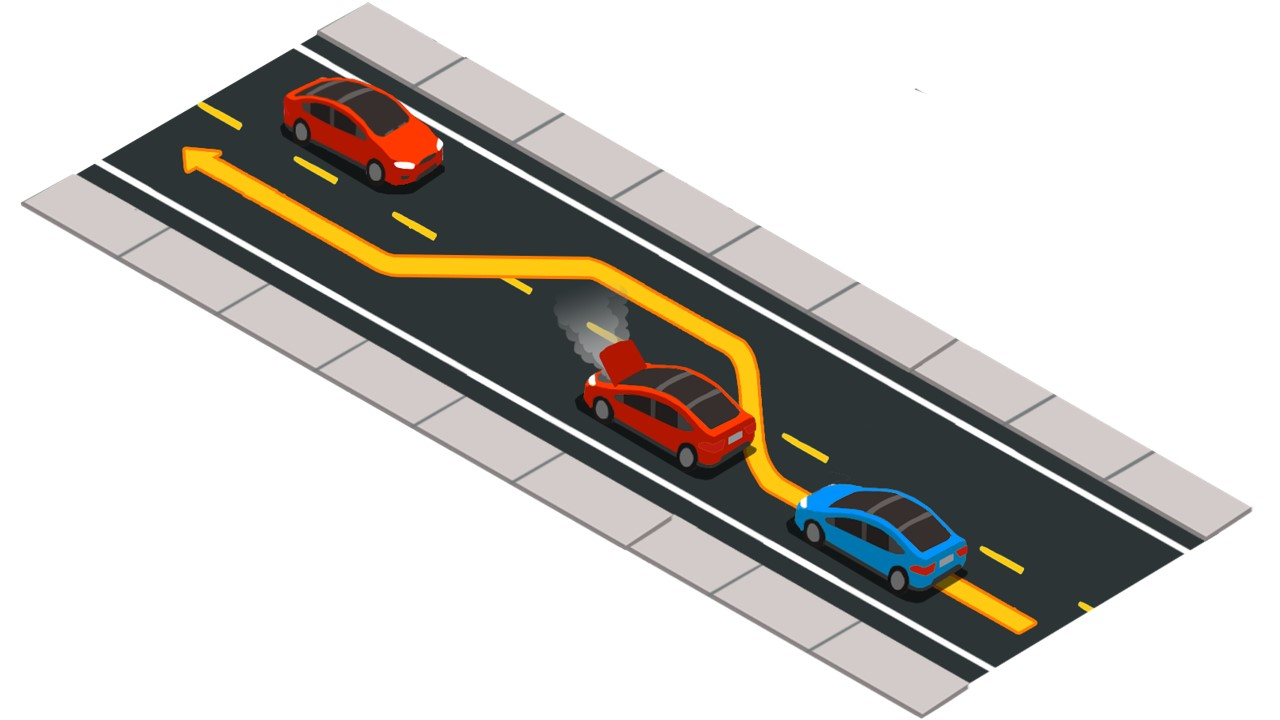
\includegraphics[width=8.5cm]{\pathToOtherFiles/figures/carla_challenge_NHTSA_task6_LHS.jpg}
%     \caption{Overtaking scenario from NHTSA~\cite{nhtsa_precrash}.}
%     \label{fig:carla_challenge_NHTSA_task6_LHS}
% \end{figure} 

%This scenario is challenging for the autonomous vehicle as there are competing goals firstly to ensure safety and avoid accidents but also to make reasonable progress along the road network given the conditions, i.e. maintain \textit{liveness}. There is also significant challenge in validating vehicle safety in such a scenario, whether in the real world or in a simulation. For the overtaking scenario several parameters need to be monitored in order to check each assertion. 

In the simulation and the real-time video analysis experiments, we chose to assess clauses in two different UKHC overtaking rules. The simulation study developed an assertion for the first bullet-item of Rule 162 (as discussed in Section \ref{interp_nat_lang_UKHC_rules} and also in Section \ref{model_based_analysis}), developing an assertion check to determine whether a Safe Distance Ahead existed for an AV performing an overtake manoeuvre on a single-lane road, as it began to cross the road centre line at the start of the manoeuvre. The real-time safety validation study developed video analysis measurements that would support assertion checks against the fourth bullet-item of Rule 163 (see Section \ref{interp_nat_lang_UKHC_rules}; the relevant clause is italicised in that section for ease of identification) - while the measurements were not developed fully into assertions in SQL code, the study does capture the information essential to the assertion hypothesis for that UKHC clause (the Cut-in Clearance distance as discussed in Section \ref{model_based_analysis}), and would be generated as a derived variable in the database using a standard procedure function as discussed previously.

\subsection{Simulation case study}  \label{sim_case_study}
In the simulation case study we developed an assertion check for Safe Distance Ahead at the start of overtaking, using the expression for SDA discussed earlier in Section \ref{model_based_analysis}. We ran the simulation using a real road map segment (of a road in Bristol, UK, part of an AV test route being considered for the ROBOPILOT project\footnote{See URL: \url{http://www.bristol.ac.uk/tsl}}).

\subsubsection{Environment model}
The map segment used for the simulation case study is shown in 
Figure~\ref{fig:assertion_database_annotated}. For the sake of simplicity we ran the simulation on one of the straight sections of road, which avoided having to take considerations such as obscuring objects or limited lines of sight into account. The road layout model was developed using the Road Runner software package, from an OpenDrive environmental model developed from Open Street Map (OSM) data obtainable freely from UK government sources (Ordnance Survey).\footnote{\url{https://os.openstreetmap.org/}} 

% \begin{figure}[htp]
%     \centering
%     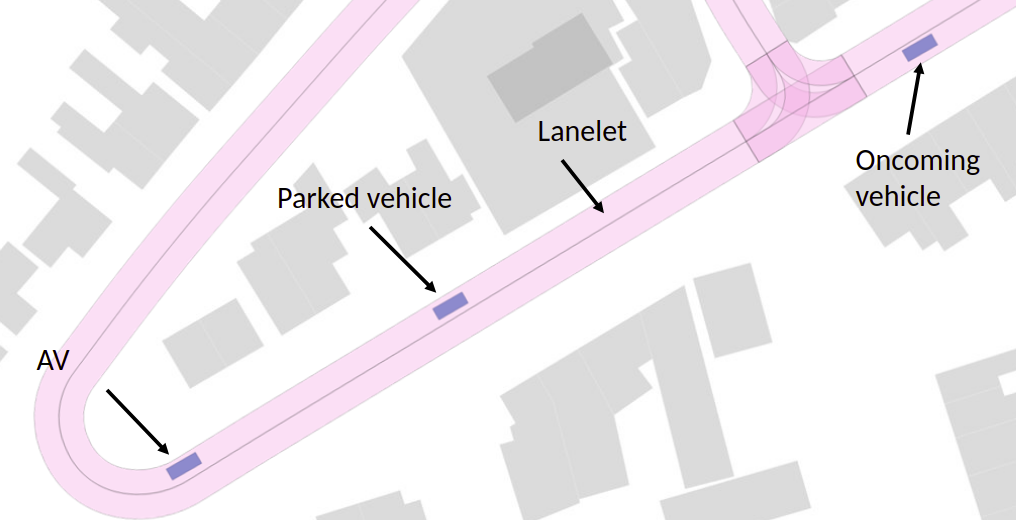
\includegraphics[width=8.5cm]{\pathToOtherFiles/figures/Lanelets_anno_av.png}
%     \caption{Lanelets overlaid onto road network.}
%     \label{fig:lanelets}
% \end{figure} 

As discussed in Section \ref{geospatial_database}, lane polygons are required for efficient measurement of vehicle lateral movement within, and partial occupancy of, road lanes; in this simulator case study we used a lane partitioning concept termed \textit{lanelets}~\cite{lanelets2014}, which allows exactly this level of description of the scene. We used an open-source software conversion package~\cite{lanelets_to_openDrive} to generate the lanelet data from the openDrive~\cite{opendrive} model, dividing the roads into individual lanes and lanelets. This data was imported into the PostgreSQL database as a table of lane segment polygon objects ($lanelets.lanelet\_shape$) covering the whole road layout used for the study. Additionally, information about lane boundaries and orientations, required to identify road orientation and running lane directions, was appended to this data. 
%
Figure~\ref{fig:assertion_database_annotated} shows an example of the lanelet shape object overlaid onto a road network. The blue boxes represent the dynamic actors, which in our case are the vehicles involved in the overtaking scenario. 
%
All of the above world map information was pre-loaded statically into the database, for use by the SQL query engine running the assertions queries, as discussed in Section \ref{generic_sim_system} and shown in Figure~\ref{fig:SimulatorArchitecture}.

\subsubsection{Overtaking Profiles} \label{overtaking_profiles}
The intent of the Safe Distance Ahead assertion we developed was to assess whether sufficient distance ahead of the simulated AV was available at the initial decision point of the manoeuvre for it to complete an overtaking manoeuvre safely. However, in practice, sufficiency of the distance ahead is dependent in part on the driving profile that the AV controller has selected to perform (see Section \ref{model_based_analysis}). But, if the safety validation exercise is to be performed as an independent 'black-box' measurement of AV behaviour (as is often the case in many practical development projects), the internal plans of the AV may be unavailable to the system testers, and we conducted our experiment in such a manner as to reflect such a situation.

%\footnote{Furthermore, it is always possible for the AV to change its profile in mid-manoeuvre, thereby shortening the remaining distance required, which can be applied as an emergency action if the risk of the situation should increase for any reason. So, the assessment whether there is a safe distance ahead in any given situation at the start of an overtake manoeuvre is dependent in part on the internal plans of the AV at the time, and must be made without full knowledge of exactly how the manoeuvre will play out after the Safe Distance Ahead assessment has been made.} 

The simulated AV in the experiment was programmed to follow a preset trajectory, which was not used to influence the choice of parameters in the Safe Distance Ahead assertion expression. We developed three different variations of the SDA assertion, each calculating the safe distance ahead using the formula developed from the modelling analysis (see Section \ref{model_based_analysis}), but which assumed three different driving profiles corresponding to three different levels of urgency of overtake manoeuvre (called `relaxed', `hurried' and `aggressive'). The levels of urgency were based loosely on similar concepts developed in other Human Factors research~\cite{Chen2015,wang2019analysis}, which had equated level or degree of urgency with \emph{Time To Collision} (TTC). These sources identified that a TTC of approximately two seconds corresponds approximately to a medium degree of urgency, which we have labelled `hurried'. These three variants of the SDA assertion were then applied to the simulation data produced by the preset AV controller to see whether which SDA situation that occurred in each simulation run was acceptable for which driving profile.

\subsubsection{Simulator system details}

The simulator used for the case study was a minimal version of the generic simulator testbench architecture described in Section \ref{generic_sim_system}. The system used the CARLA simulation software \cite{CarlaSimulator}, an open-source autonomous driving simulation environment. Dynamic state data generated by the simulator was passed to a PostgreSQL database as shown in Figure~\ref{fig:SimulatorArchitecture}, with the SQL assertion script being applied in retrospective analysis mode as discussed in Section \ref{Assertions_at_Sim_Time}.

The paths followed by each simulated vehicle (AV, VBP, OV - see Figure~\ref{fig:assertion_database_annotated}) were preset to follow a series of way-points. Using fixed vehicle paths facilitates evaluation of the assertion, as it made the test repeatable\footnote{Test repeatability is needed to ensure trust in the simulated assertion results and also to ensure software bugs are found and fixed efficiently. Repeatability relies on deterministic simulation code and hardware. If the \emph{simulation variance} is within tolerance then verification coverage results are stable and if an assertion fails the test can be re-run to provide the same output as described in~\cite{chance2021}.} and allowed us to see how different characteristic parameters affected the assertion checking (see Section~\ref{sim_results} for details). 

CARLA generates dynamic state information about the simulation actors (vehicles), which is made available via an API, and Python scripts were written to transfer data from the simulator into the PostgreSQL database on a step-by-step basis.

\subsubsection{Simulation runs}

Three simulation runs were executed to generate simulation data traces for assessment by assertion checking. In each case, the trajectory of the AV remained unchanged, overtaking the stationary VBP and cutting back into the running lane with the same pull-out and cut-in clearance distances each time. The OV trajectory simply moved along the oncoming lane at constant speed, but the starting position of the Oncoming Vehicle was varied so as to generate three different scenarios of i) a safe overtake manoeuvre, ii) a near miss and iii) a dangerous overtake manoeuvre resulting in a collision. The simulation data was logged and transferred into the assertion database as three distinct subsets of samples within the main captured data tables. These were then analysed retrospectively after the end of the simulation run, using assertions designed to assess whether (and how well) the AV performed overtake manoeuvres of differing profiles (as discussed in Section \ref{model_based_analysis}). These results are discussed below.

\subsubsection{Simulation Assertion Checking Results} \label{sim_results}
In this section we discuss the outcomes of the simulation safety validation analysis, and the implications on the methodology of developing and using assertions.

The three simulation runs described previously produced simulation data logs that were subjected to assertion checking to ensure that a safe distance ahead existed as the AV began to cross the road centre line into the oncoming lane at the start of the overtake manoeuvre. However, there are several factors conditioning the test results that need to be taken into account.

Comparison of the three variations of test against the simulated scenarios (safe, near miss and collision) produces nine distinct tests. 

The fixed overtaking manoeuvre trajectory that had been pre-set for the AV vehicle approximated to a medium level of urgency, in terms of the pull-out and cut-in clearance distances achieved (about 2s time to collision at the simulated speeds of the vehicles). This meant that for a set of tests having a range of urgency levels centred on the medium urgency case, one should get a sliding scale of test case passes and failures as the test case variants are applied to decreasing initial separation distances between AV and OV in the three simulation logs. The results of the tests are shown in Table \ref{Overtaking_Profiles}, which shows the required separation distances at the start of each manoeuvre (determined by the modelling analysis formula described in Section \ref{model_based_analysis}), the Distance Ahead that was achieved in each simulation run, and thence the pass/fail assertion results of comparing the two distances in each case.

\begin{table}[h]
\centering
\begin{tabular}{lcccc}
\hline
\\
\multirow{3}{*}{\textbf{Scenario}} & \textbf{Achieved} & \multicolumn{3}{c}{
\textbf{Distance Ahead required by profile (m)}}\\ %GC edit for arxiv
% \textbf{Distance Ahead required (m)}}\\
& \textbf{Distance} & `Relaxed' & `Hurried' & `Aggressive' \\
& \textbf{Ahead (m)} & 101.39 & 63.73 & 40.02 \\
\\
%
Safe & 76.43 & FAIL & Pass & Pass\\
%
Near miss & 58.33 & FAIL & FAIL & Pass\\
%
Collision & 35.63 & FAIL & FAIL & FAIL\\
\\
\hline
\end{tabular}
\caption{Pass/Fail Assertion results.} \label{Overtaking_Profiles}
\end{table}

The table shows that it would have been inadvisable to perform a `relaxed' overtake in any of the three scenarios presented, as this would have resulted in a near miss or a collision. If a `hurried' overtake is attempted (which actually corresponds to the behaviour of the AV in the scenarios), this policy was acceptable for the `Safe' scenario, but inadvisable for the `Near Miss' and `Collision' scenarios (as their descriptive names imply). And if the AV had been programmed to overtake aggressively in these scenarios, then only in the case of the Collision scenario circumstances would the Distance Ahead have been short enough for the manoeuvre to be inadvisable; in the other two cases the overtake could have been achieved successfully (although aggressive overtaking may result in other safety assertions being violated).

\subsection{Runtime case study}
In the runtime case study we developed an assertion monitoring for checking safe stopping distance during the overtake. 
%
To demonstrate the use of assertions at runtime monitoring of an AV, in the absence of a fully functioning AV controller, we used manual video analysis in combination with a pre-trained object classifier to extract data from a dashboard video camera of a dangerous overtaking vehicle.\footnote{Link to video used in analysis: \url{https://youtu.be/Gzi4X7WZkRI}.} 
%
The aim of the assertions applied to runtime data was to assess whether the AV risks colliding with any of the other vehicles involved in the scenario during the overtake and in turn take an informative decision on aborting or continuing the overtake. 
%
Such situations are very likely to happen if road layouts are more complex, vehicles change speed or if for any other reason the SDA calculation at the start of the manoeuvre gives misleading estimates. 

\subsubsection{Danger Space (DS) Assessment}
\label{DS_assessment}

The overtake manoeuvre can be split into three distinct stages as was described in the modelling analysis (Section \ref{model_based_analysis}): pulling out, passing VBP and cutting in.
%
During the different stages of the overtake, non of the vehicles should be present in the DS of another vehicle nor should the DS of one of the vehicles overlap with the DS of another. 
%
To satisfy this requirement, six assertions are needed to be checked at the different stages of the overtake.
%
The subscript DS will be used to refer to a vehicles danger space.

The first four assertions are applicable through out the three stages of the overtake, these are:

\noindent \textbf{i)} the VBP should not be in the AV danger space at anytime during the overtake, 

\noindent \textbf{ii)} the OV should not be in the AV$_{DS}$, 

\noindent \textbf{iii)} the AV should not be in the OV$_{DS}$, 

\noindent \textbf{iv)} there should be no intersection between the AV$_{DS}$ and OV$_{DS}$.

There are two key SPIs applicable for the last stage of the overtake (cutting in):

\noindent \textbf{v)} the AV should not enter the VBP$_{DS}$ and 

\noindent \textbf{vi)} there should be no intersection between the AV$_{DS}$ and the VBP$_{DS}$. 

\subsubsection{Video analysis}
%
Usually well trained machine learning models are used with stereo vision and information from other sensors, like LIDAR, odometers etc, to estimate accurately the position, orientation and velocities of the AV and surrounding static and dynamic objects.
%
However, due to the absence of a fully functioning AV, we used the following approach to approximate the processing of the real-time data stream for the runtime case study:

First, a pre-trained object classifier, YOLOv3~\cite{Yolo}, was used to provide locations of vehicles in each frame and how much area each vehicle occupies of the frame. 
%
The separation distances between the AV and the other vehicles are the SPIs at the various stages of the overtaking manoeuvre. 
%
The longitudinal distance ($s$) of a vehicle along the road from the AV can be estimated 
using Equation~\ref{s_equation}:
\begin{equation}\label{s_equation}
    s = \frac{c\times W}{w}
\end{equation}
where $c$ is a constant capturing the focal length of the camera and is found empirically, $W$ is the actual width of a vehicle in meters, and $w$ is the width of the box detected by YOLOv3 in pixels.

Second, the lateral distance $d$ of the AV from the middle white line is estimated using Equation~\ref{d_equation}: 
%
\begin{equation}\label{d_equation}
    d = \frac{w_{L (real)}}{w_{L (pixels)}} \times d_{pixels}
\end{equation}
%
where $w_{L (real)}$ is the real lane width measured in meters, $w_{L (pixels)}$ is the lane width measured in pixels and $d_{pixels}$ is the lateral distance of the AV from the middle white line in pixels. $d_{pixels}$ is determined by simply finding where the middle white line is compared to the middle of the frame. The VBP and OV are assumed to have a fixed lateral distance from the white line separating lanes. Third, the pull out $\beta$ and cut in $\theta$ angles of the AV are calculated using the change in lateral distance and change in the longitudinal distance measured. Fourth, as we were not able to measure vehicle speed directly from the video, we based the DS calculation on the worst case scenario; that is all vehicles were traveling at the speed limit of the road. The speed limit of the single carriage way in the video was found to be the national speed limit. According to Rule 124 in the UKHC the national speed limit for cars (AV and OV) is 60mph, and 50mph for goods vehicles (VBP). Using the above steps the real time video was converted to a 2D driving scenario, where the danger space assertions listed in section~\ref{DS_assessment} can be checked.

\subsubsection{Runtime Validation Results}
Table~\ref{Overtaking_DS_table} shows the results for the six assertions introduced in section~\ref{DS_assessment} at the three different stages of the overtake. At pulling out, the assertion checks suggest that it was safe to continue the overtake manoeuvre as non of the vehicles were present in another vehicles danger space and there was no overlap in any of the danger spaces. 
When passing the VBP the assertion checks indicate that the overtake should have been aborted or if it was aborted then it should have been aborted earlier during passing the VBP stage as both the AV and the OV have entered each others danger spaces. Finally at the last stage of the overtake, the assertion checks suggest that the AV has attempted to cut in before it has completely overtaken the VBP, whilst still failing the assertions relating to the OV. However, the AV has passed the assertion of not being in the VBP$_{DS}$, which suggests, given all of the other assertions have failed, that it has not overtaken the VBP before cutting in.

\begin{table}[h]
\centering
\begin{tabular}{ lcccc }
\hline
\\
\multirow{3}{*}{\textbf{}} & \multicolumn{3}{c}{\textbf{Overtaking manoeuvre stages}}\\
\textbf{Assertion} & \textbf{Pulling out} & \textbf{Passing VBP} & \textbf{Cutting in} & \\
&  &  &  & \\
VBP not in AV$_{DS}$ & PASS & PASS & FAIL\\
%
OV not in AV$_{DS}$ & PASS & FAIL & FAIL\\
%
AV not in OV$_{DS}$  & PASS & FAIL & FAIL\\
%
No AV$_{DS}$ $\cap$ OV$_{DS}$  & PASS & FAIL & FAIL\\
%
AV not in VBP$_{DS}$  & N/A & N/A & PASS\\
%
No AV$_{DS}$ $\cap$ VBP$_{DS}$  & N/A & N/A & FAIL\\
%
\\
\hline
\end{tabular}
\caption{Pass/Fail danger space assertion checks results.} \label{Overtaking_DS_table}
\end{table}

\section{Discussion} \label{discussion}

\subsection{Assertion Checking to measure Performance}
While we have applied the assertion checking methodology to measure the safety properties of vehicles in simulation and at runtime, the methodology can be extended to other important system engineering aspects as well. This may include performance based metrics such as smooth driving (minimal jerk), accuracy of control (such as parking or stopping precisely at a bus stop), and decisive behaviour at junctions or roundabouts, sometimes termed \emph{liveness}~\cite{kim2014mpc}. In particular, the mission performance of a vehicle, for example, can be measured in journey time or efficiency of movement through traffic, which may affect not only passenger expectations but also the commercial viability of such an autonomous system. 

Performance (achievement of task goals) and safety (avoidance of task hazards) are distinct behavioural properties of a system; achievement of one does not entail achievement of the other. A task controller must achieve satisfactory compliance with both properties if a dependable system is to be developed. In some scenarios, such as during overtaking, their may exist a competition within the controller to satisfy both the achievement of goals and the avoidance of hazards. 

For example, an autonomous taxi may need to perform a minimum number of fare-paying journeys in a day in order to remain commercially viable. Performance assertions can measure whether suitable opportunities for manoeuvres such as overtaking were taken efficiently, without incurring delays or driving sub-optimally for the given road network i.e. using all available space. However, it must still drive safely as it conducts each journey, so in situations that may induce journey delays, such as high traffic congestion, optimum performance and safety may not be mutually achievable. Assertions can measure how the AV trades off these two properties in the execution of its task(s).

An analysis for overtaking performance can be observed in the simulation results presented in Section~\ref{sim_case_study} by comparing the required SDA to the actual distance ahead of the Oncoming Vehicle as listed in Table~\ref{Overtaking_Profiles}. In this previous example, a failure of the SDA assertion indicates a violation of the UKHC and this happens when the actual distance ahead is less than the required Safe Distance Ahead, i.e. intersecting the danger space of the Oncoming Vehicle. Considering this example from the point of view of performance, the AV must not violate the safety property but must overtake within a reasonable window of opportunity ($\delta$), i.e. taking any presented opportunity to overtake if safe to do so and if appropriate to the road network. We define $\delta$ as the ratio of `achieved distance ahead' to the `SDA required by profile' from Table~\ref{Overtaking_Profiles}. The size of this \emph{opportunity window} will be dependent on a myriad of different contextual and preferential conditions such as the driving style, vehicle capability, passenger comfort, etc. 

Table~\ref{performance_metric_table} shows the classification for the overtaking scenario but from the perspective of performance rather than safety. There are three conditions in Table~\ref{performance_metric_table} describing the distance to the Oncoming Vehicle with respect to required SDA and the opportunity window. 
\begin{enumerate}[1)]
    \item Unsafe: $d_{OV} < SDA$
    \item Higher Performance: $SDA \leq d_{OV}$ $\leq SDA.\delta$
    \item Lower Performance: $d_{OV} > SDA.\delta$
\end{enumerate}
%
Here, $d_{OV}$ is the distance to the Oncoming Vehicle, SDA is the required Safe Distance Ahead based on the model given in Appendix~\ref{appendix_a} and the ratio $\delta$ is the optimal window of opportunity for the vehicle to perform the manoeuvre. For condition 1, the distance to the Oncoming Vehicle is less than SDA, so to not overtake is the only safe action and indeed to overtake in this condition would result in the SDA safety assertion failure. Safe driving behaviour whilst making timely use of the overtaking opportunities presented to the vehicle will see the vehicle progress through traffic most efficiently. This sentiment is captured in condition 2, where the vehicle is taking opportunities to overtake whilst maintaining a safe distance to the oncoming vehicle. In condition 3, the distance to the Oncoming Vehicle is greater than $SDA$ plus the window of opportunity, where the vehicle has unhindered opportunity, i.e. no currently oncoming traffic. In this case not overtaking, although completely safe, will incur unnecessary delay to the journey and may be given a lower performance score. Overtaking in this condition would be the expected behaviour of the AV and as such could be assigned a neutral or small positive performance score.

\begin{figure}[t]
    \centering
    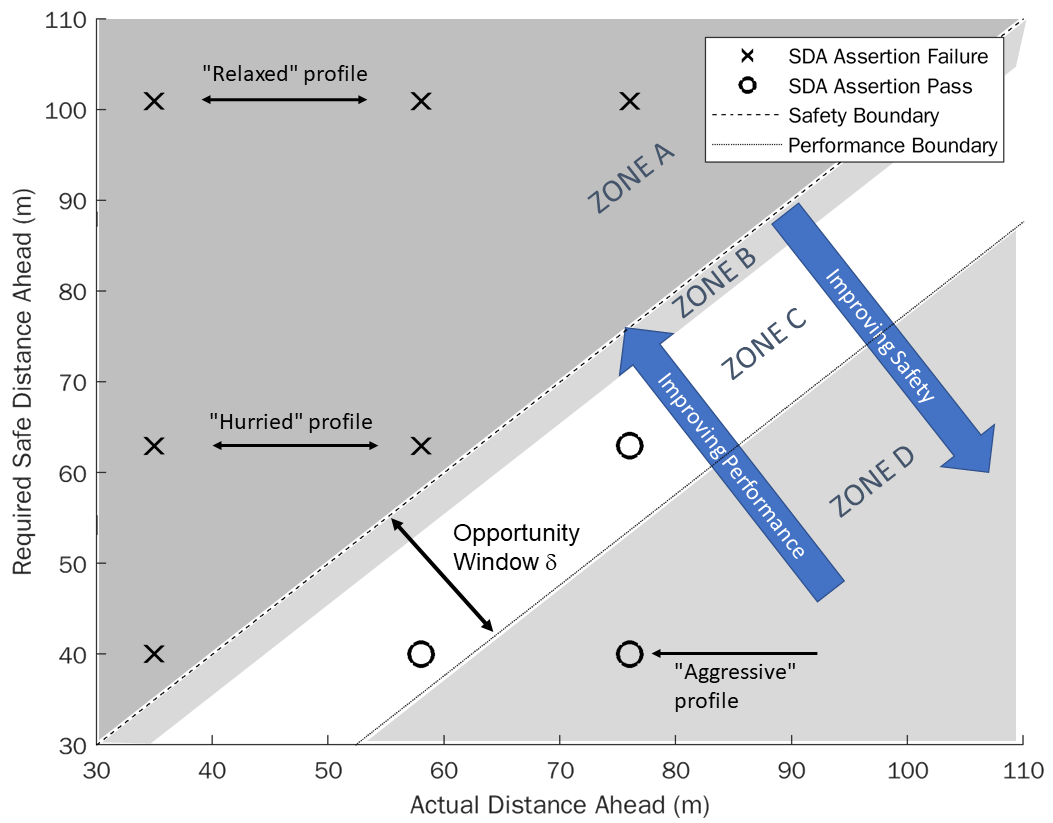
\includegraphics[width=8.5cm]{\pathToOtherFiles/figures/SDA_annotated.png}
    \caption{Simulation results for performance.}
    \label{fig:performance_results}
\end{figure}

The previous simulation results from the perspective of performance are shown in Figure~\ref{fig:performance_results}. Here $\delta$ is set to be equivalent to TTC=$2.5s$ \cite{Robbins2018,Chen2015,wang2019analysis} for the purposes of illustrating this concept. The required SDA is shown as a function of the actual distance ahead for the three overtaking profiles. Unsafe test cases are shown as cross markers, all being within \emph{Zone A} which is an area where the SDA assertion will be violated. At the edge of this area defining unsafe driving behaviour is a \emph{safety boundary} (dashed line) being the edge of Zone A. Beyond the safety boundary exists the opportunity window that extends to the limit of the \emph{performance boundary} (dotted line), and covers \emph{Zone B} and \emph{Zone C}. Zone B represents a conceptual \emph{safety margin} or \emph{buffer} between optimal performance and the safety boundary, and in reality this may be the limit of a near-miss condition, e.g. TTC=$0.5s$. Reward should be given for an adaptive controller that makes use of Zone C but does not enter Zone B, i.e. executes optimal overtaking given opportunity $\delta$ but does not cause a near-miss event. \emph{Zone D} can be considered safer than the other zones, i.e. the vehicle is giving lots of distance to the Oncoming Vehicle, but may be unnecessarily incurring delays and hence considered lower performance. An improvement could be made by moving from Zone D to Zone C without violating any safety property. 

There is therefore a trade-off between safety and performance for optimal driving behaviour, where performance is improved by moving towards Zone B (but not passing the safety boundary), and safety is improved by moving towards Zone D (see large arrows in Figure~\ref{fig:performance_results}). While we have observed this conceptual trade-off between safety and performance in our analysis, we also see evidence of this in the UKHC rules themselves. An example of this is exemplified in the 4th bullet point in Rule 163 (see Section~\ref{interp_nat_lang_UKHC_rules}) where the overtaking rule states ``Move back to the left as soon as you can but do not cut in", which clearly suggests that performance will play a part in correct driving behaviour. There is also evidence of this trade-off between performance and safety, while the AV should complete the overtake maneuver ``as soon as you can" (higher performance) but ``do not cut in" (higher safety) we see these competing demands resolve in optimal driving behaviour analogous to that described by Zone C in Figure~\ref{fig:performance_results}. This analysis considers only the overtaking scenario and in reality there will be many competing demands on the decision making process of a real controller. 

\begin{table}[]
\centering
\begin{tabular}{|p{2.3cm}|p{2.3cm}|p{2.3cm}|}
\hline
\multicolumn{1}{|l|}{Distance Ahead} & \multicolumn{1}{l|}{\textbf{AV Does Not }} & \multicolumn{1}{l|}{\textbf{AV Overtakes}} \\ 
Condition & \textbf{Overtake} & \\
\hline
\multirow{2}{*}{1: Unsafe} & safe & unsafe (assertion \\
& & failure) \\
\hline
\multirow{2}{*}{2: Higher} & safe but not taking & safe and taking\\ 
      Performance & opportunities & opportunities\\
\hline
\multirow{2}{*}{3: Lower} & safe but incurring  & safe \& expected  \\ 
Performance & significant delay & behaviour\\
\hline
\end{tabular}
\caption{Performance classifications for deciding to overtake based on the distance ahead to the Oncoming Vehicle.}
\label{performance_metric_table}
\end{table}


% \begin{figure}[ht!]
%     \centering
%     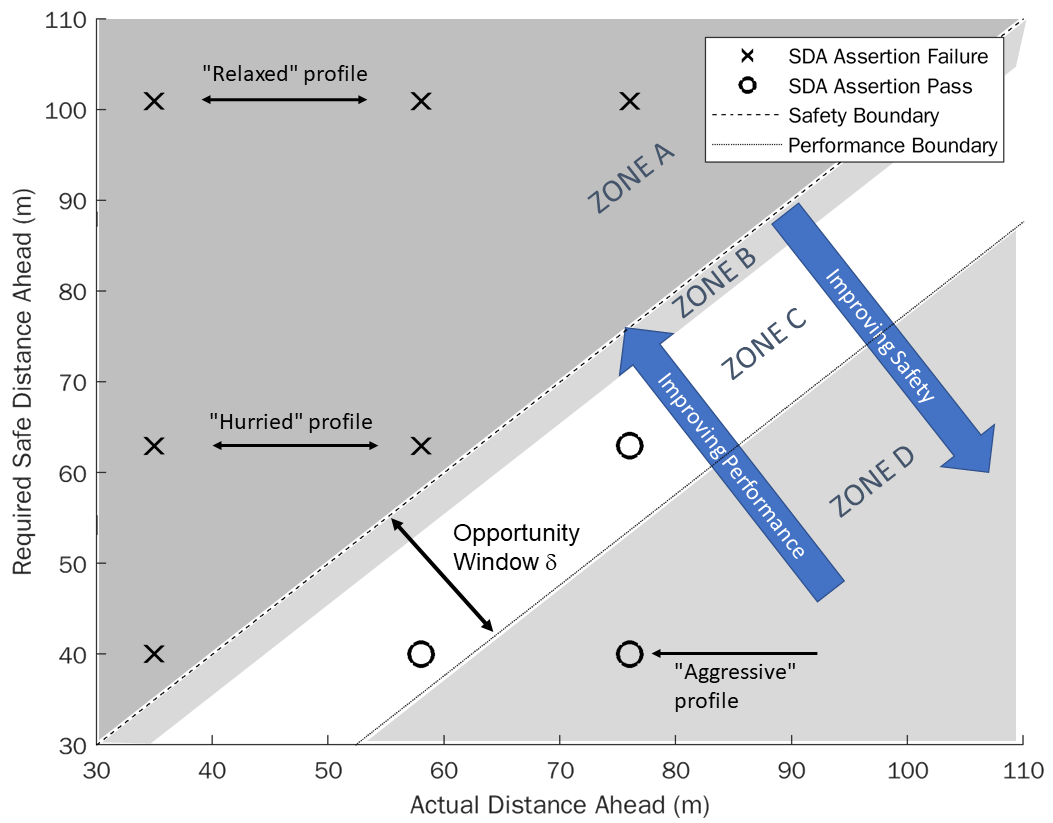
\includegraphics[width=8.5cm]{\pathToOtherFiles/figures/SDA_annotated.png}
%     \caption{Simulation results for performance.}
%     \label{fig:performance_results}
% \end{figure}

% \subsection{The Significance of Agent Intentions during Assertion Checking} %in Defining Validation Cases} \label{discussion_of_results}
\subsection{Agent Intentions during Assertion Checking}
The initial work presented in this paper has raised a number of consequent issues that require further investigation. One significant topic is the extent to which assertions require access to states of internal decision making within the autonomous vehicle being monitored. Many UKHC rules are advisories to %drivers or other road users to be aware of 
potentially hazardous situations, and to actively perceive, deliberate, and take special or particular action to avoid harmful events. 
% 
% GC think we should just focus on one or two of these points
An excerpt from Rule 146 of the UKHC states \begin{quote} \textit{Try to anticipate what pedestrians and cyclists might do. If pedestrians, particularly children, are looking the other way, they may step out into the road without seeing you.} \end{quote} which specifically asks to perceive and anticipate future developments of the situation. If we want to validate the correctness of an AV's behaviour in respect of these rules we must have the capability to observe the decisions made by the AV or its control system as they are made. 





% GC Removed this ***
% The following extracted rule is an example:
% \begin{quote}
%     \textit{
%     \textbf{Rule 146}
%     \textbf{Adapt your driving} to the appropriate type and condition of road you are on. In particular
%     \begin{itemize}
%         \item do not treat speed limits as a target. It is often not appropriate or safe to drive at the maximum speed limit
%         \item take the road and traffic conditions into account. Be prepared for unexpected or difficult situations, for example, the road being blocked beyond a blind bend. Be prepared to adjust your speed as a precaution
%         \item where there are junctions, be prepared for road users emerging
%         \item in side roads and country lanes look out for unmarked junctions where nobody has priority
%         \item be prepared to stop at traffic control systems, road works, pedestrian crossings or traffic lights as necessary
%         \item try to anticipate what pedestrians and cyclists might do. If pedestrians, particularly children, are looking the other way, they may step out into the road without seeing you.
%     \end{itemize}
%     }
% \end{quote}
% % Each of the bullet-items listed above would probably require at least one distinct test case (often more than one). But several items
% Several bullet-items listed above ask the road-user to consider particular situations explicitly, advising that increased attention or effort be put into the perception of particular conditions, features of, or objects in the environment (e.g. blind summits, pedestrians, unmarked junctions). If we want to validate the correctness of an AV's behaviour in respect of these rules we must have the capability to observe the decisions made by the AV or its control system as they are made. 

This case highlights the need for \emph{explainable AI}, a topic gaining increasing attention in the AI, robotics and autonomous systems community. The opinion is widely held \cite{deeks2019judicial, o2019legal, wortham2020transparency} that it may be essential for any such system employed in a safety related application to be able to explain its decision making. The complexity and opacity of internal functional representations in many AI technologies, combined with the non-deterministic nature of complex operational situations in real world environments means that they may not be repeatable in post-incident analysis without the system being able to report the precise situation that it perceived, and the planning or action-selection decisions that it made as a consequence. This requires some form of communication protocol or interface from the decision-making centres of the system to the outside world, so that the decisions can be observed and recorded for later analysis. This is a significant motivation behind the use of an assertion-based oracle subsystem as a runtime analysis facility, discussed in Section \ref{assertions_at_run_time}.

At present, we are not in a position to perform assertion checking for this kind of safety property by means of an independent assertion-based oracle. There is no externally objective way to observe whether an AV agent is actually performing deliberative reasoning, planning or action selection consistent with rules such as Rule 146, unless it communicates explicitly its planning and decision-making through an interface, whose information can be read by the oracle for checking. A standard protocol for reporting decision-making information would need to be developed and at time of writing no such standard for doing this has been agreed. And given the commercially sensitive nature of such information, we do not anticipate that manufacturers would be willing to design systems that volunteer such information without legal requirements to do so and a standard protocol to use.

In the absence of any such explanation capabilities or facilities, it is still possible to achieve some degree of validation by performing checks derived from the text of the rule, which attempt to challenge the hypothesis expressed or implied by the UKHC rule or rule clause (\emph{e.g. falsification testing}) of the safety property. For example, in the testing phase of an AV, to exercise the last bullet item of Rule 146 above one could construct a test case, perhaps similar in nature to those defined in \cite{EuroNCAP}, where simulated `children agents' (that model the physical appearance of children as well as some aspects of their behaviour) step out into a road in front of the AV agent, having appeared either to be looking away from an AV agent, towards it, or some mix of the two focuses of attention. Such a test suite could then test the capability of the AV control system to evaluate the potential behaviour of children to determine what driving action can be taken successfully and safely. This can test the `end-to-end' situated behaviour of the vehicle and thereby evaluate the cumulative effect of decision making, but as evidence to support a safety case this is less effective than explicit confirmation (by recording) of the AV's decision process that would come from Explainable AI.

\section{Conclusion}\label{conclusion}
The results obtained from both the simulation and the runtime video analysis case studies show the general feasibility and utility of assertion-based safety validation testing, with the assertions being derived from regulatory documentation written in natural language and intended for human drivers rather than written specifically to be usable by computer. The results provide our first indication that human-oriented natural language rules of driving are an effective oracle for assessment of artificial systems.

The case studies were carried out at an early stage of development so we did not employ every element of the methodology that has emerged. Nevertheless, we believe that enough of the process has been demonstrated to show that the full methodology is viable. We also present the idea of using UKHC-based assertion checking methodology as a method to infer autonomous vehicle performance and have demonstrated this with an overtaking scenario using simulation results. We have demonstrated that a common UKHC assertion-based oracle is equally usable in runtime monitoring as it is in simulation.


% GC condensed this section:
% \subsection{Future Work}\label{future_work}
We are considering numerous other directions in which to continue this work such as extending the sources of information for safe driving, e.g.\ German driving regulations~\cite{acountability}, and models such as the RSS model \cite{RSS_Shalev_Shwartz2017,RSS2_Koopman2019}. We are also researching the use of the testbench to perform falsification testing \cite{corso2020survey, akazaki2017causality} and \emph{situation coverage testing} \cite{alexander2015} and how other techniques such as \emph{Environmental Survey Hazard Analysis}~\cite{harper2021towards} can be used to support the tool chain framework. We also aim to investigate assertion checking to provide reward function scores as a critic in reinforcement learning for continuous improvement of the AVs balance between safety and liveness during operation.



% GC removed
% \subsection{Future Work}\label{future_work}
% In addition to the ongoing work of development of the BRL Simulator Testbench, we are considering numerous other directions in which to continue this work:
% \begin{itemize}
%     \item The assertions database can be extended to other sources of information regarding safe driving behaviour of vehicles. This can include the rules and regulations of countries other than the UK (such as the German study described in \cite{acountability}), or models such as the RSS model \cite{RSS_Shalev_Shwartz2017,RSS2_Koopman2019}.
    
%     \item We are studying how the simulation testbench can be used to perform scenario-based validation methodologies such as falsification testing \cite{corso2020survey, akazaki2017causality} or \emph{situation coverage testing} \cite{alexander2015}. We are exploring how other scenario-based safety assurance techniques such as \emph{Environmental Survey Hazard Analysis}  \cite{harper2021towards} can be used to generate systematically comprehensive test objectives, scenarios and specific test cases, to produce a comprehensive safety validation methodology and supporting tool chain framework.
    
%     \item We aim to investigate and extend the use of assertion checking to provide scores as a critic or reward function in reinforcement learning processes. Allowing for continuous improvement of the AVs balance between safety and liveness during operation.
%     \end{itemize}

\section{Acknowledgments}
This research has in part been funded by the ROBOPILOT and CAPRI projects. Both projects are part-funded by the Centre for Connected and Autonomous Vehicles (CCAV), delivered in partnership with Innovate UK under grant numbers 103703 (CAPRI) and 103288 (ROBOPILOT). This research was also supported in part by the UKRI Trustworthy Autonomous Systems Node in Functionality under grant number EP/V026518/1. Also special thanks to S\'everin Lemaignan.
